\section{Hệ thống hiện tại}\label{sec:he-thong}

\subsection{Kiến trúc tổng thể}

Nhóm chia hệ thống thành 04 project (Hình~\ref{fig:overview}). Trình duyệt vào \texttt{web}, đăng nhập qua Keycloak và gọi \texttt{api} bằng Bearer token. \texttt{api} và 03 worker dùng chung 01 cơ sở dữ liệu TimescaleDB. \texttt{text2sql} là thành phần Text2SQL của Wappi, được gọi cho mọi câu hỏi dữ liệu tự do. \texttt{nilm-eval} là dự án nghiên cứu NILM, nơi nhóm huấn luyện và đánh giá mô hình trước khi đưa vào ứng dụng. Toàn bộ chạy bằng Docker Compose, dựng bằng một lệnh \texttt{./setup.sh}.

\begin{table}[!ht]
\centering\caption{Các nhóm project trong hệ thống.}\label{tab:projects}
\small\setlength{\tabcolsep}{4pt}\renewcommand{\arraystretch}{1.15}
\begin{tabularx}{\linewidth}{|>{\raggedright\arraybackslash}p{2.3cm}|>{\raggedright\arraybackslash}p{5.4cm}|>{\raggedright\arraybackslash}X|}
\hline
\textbf{Project} & \textbf{Công nghệ} & \textbf{Vai trò}\\
\hline
\texttt{web} & Next.js 16, React 19, monorepo pnpm và Turborepo, shadcn/ui & Dashboard, trang giới thiệu, giao diện đăng nhập Keycloak\\
\hline
\texttt{backend} & FastAPI, SQLAlchemy 2, TimescaleDB trên PostgreSQL 18, pgvector, Keycloak 26.2 & API 09 mô-đun, 03 worker (\texttt{replay}, \texttt{insight}, \texttt{nilm}), trợ lý Wappi\\
\hline
\texttt{text2sql} & FastAPI, LangGraph, Qdrant, PostgreSQL 17 & Lõi Text2SQL của Wappi: trả lời câu hỏi dữ liệu bằng ngôn ngữ tự nhiên, chỉ đọc dữ liệu của một nhà\\
\hline
\texttt{nilm-eval} & PyTorch, Docker (suy luận CPU) & Huấn luyện và đánh giá NILMFormer và 2Stage (mục~\ref{sec:nilm})\\
\hline
\end{tabularx}
\end{table}

\begin{figure}[H]\centering
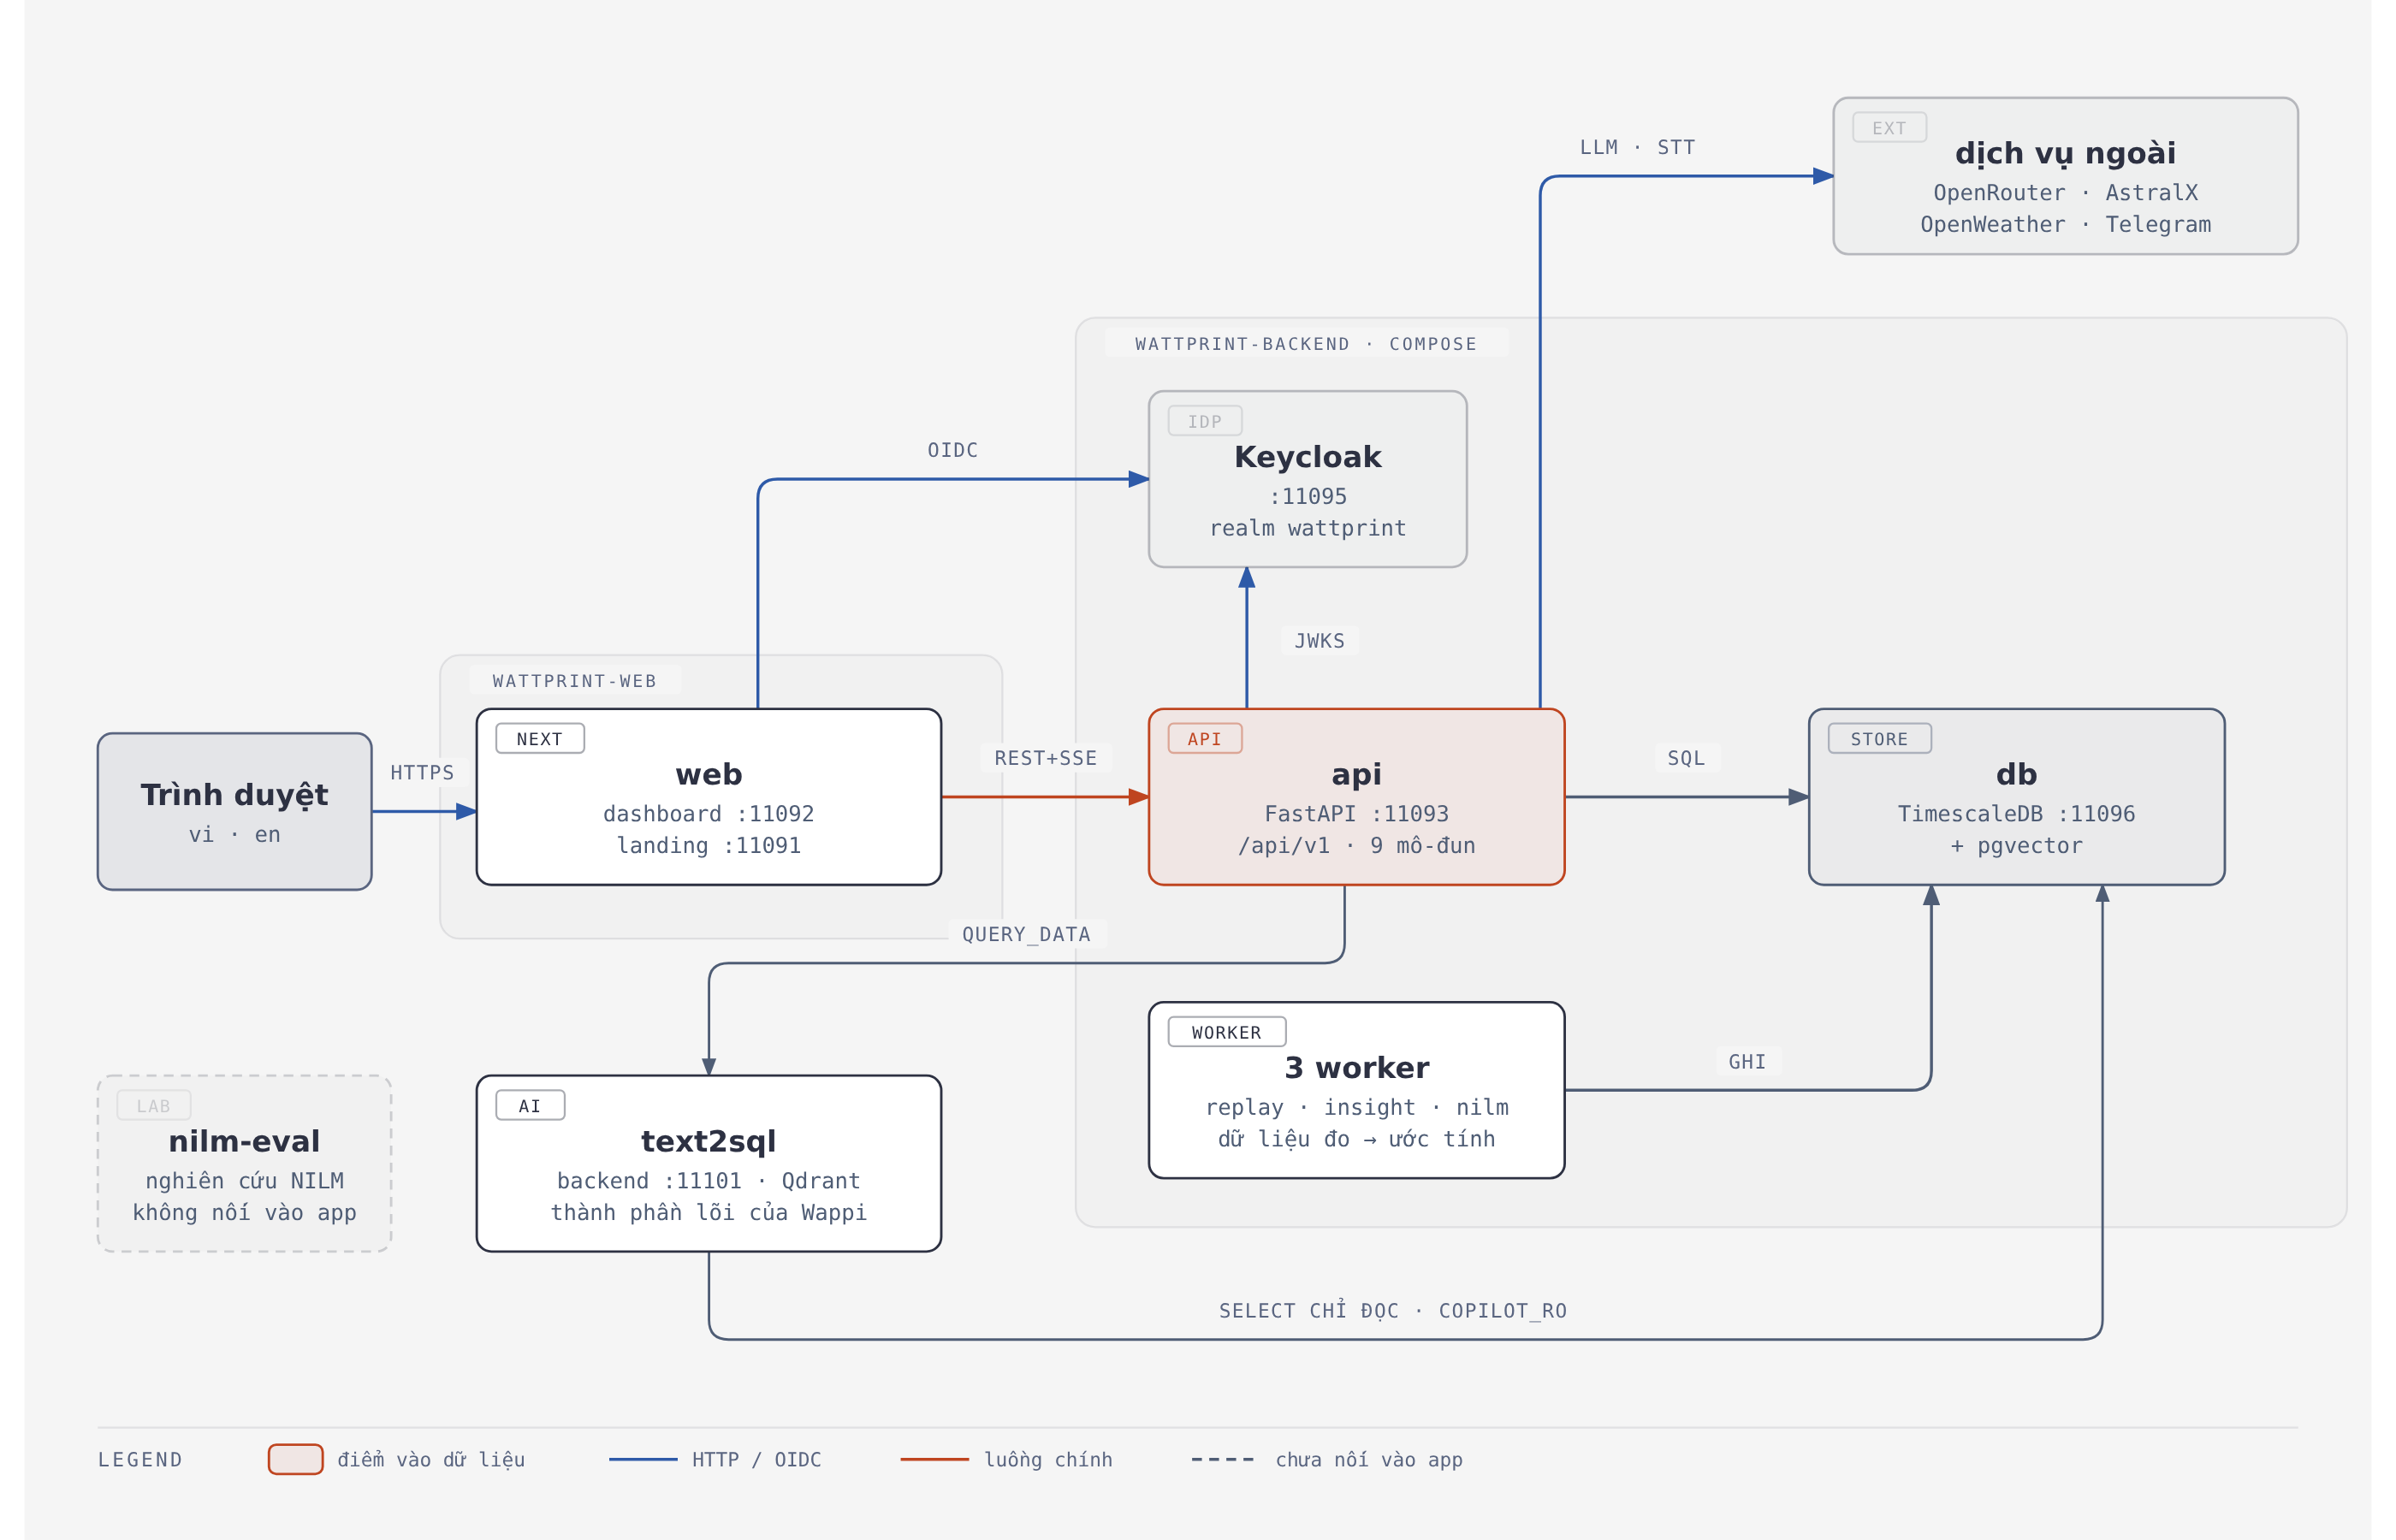
\includegraphics[width=.78\linewidth]{figures/dg_overview_t.png}
\caption{Kiến trúc đang chạy. Nét đứt là dự án chưa nối vào ứng dụng.}\label{fig:overview}
\end{figure}

\subsection{Công nghệ lõi theo từng nhóm}

\paragraph*{Backend và dữ liệu.}
Backend là một ứng dụng FastAPI chia thành 09 mô-đun (\texttt{auth}, \texttt{home}, \texttt{energy}, \texttt{billing}, \texttt{expect}, \texttt{insight}, \texttt{copilot}, \texttt{nilm}, \texttt{ops}). Một mô-đun chỉ gọi mô-đun khác qua \texttt{api.py} của nó, và một script kiểm tra ranh giới này. Số đo vào bảng \texttt{tb\_reading} (hypertable của TimescaleDB) qua một đường nạp duy nhất. Các màn hình đọc bảng tổng hợp liên tục theo phút, giờ và ngày. 03 worker chạy nền. \texttt{replay} phát lại số đo của nhà demo như công tơ thật, mỗi 5 giây. \texttt{nilm} tách điện từng thiết bị. \texttt{insight} tính hóa đơn, dự báo, cảnh báo và kế hoạch tiết kiệm. Hóa đơn tính theo biểu giá của Quyết định 2892/QĐ-BCT \citep{bct2026}. Biểu giá được lưu theo phiên bản có ngày hiệu lực, nên đổi giá hoặc thuế chỉ cần thêm một dòng dữ liệu.

\begin{figure}[H]\centering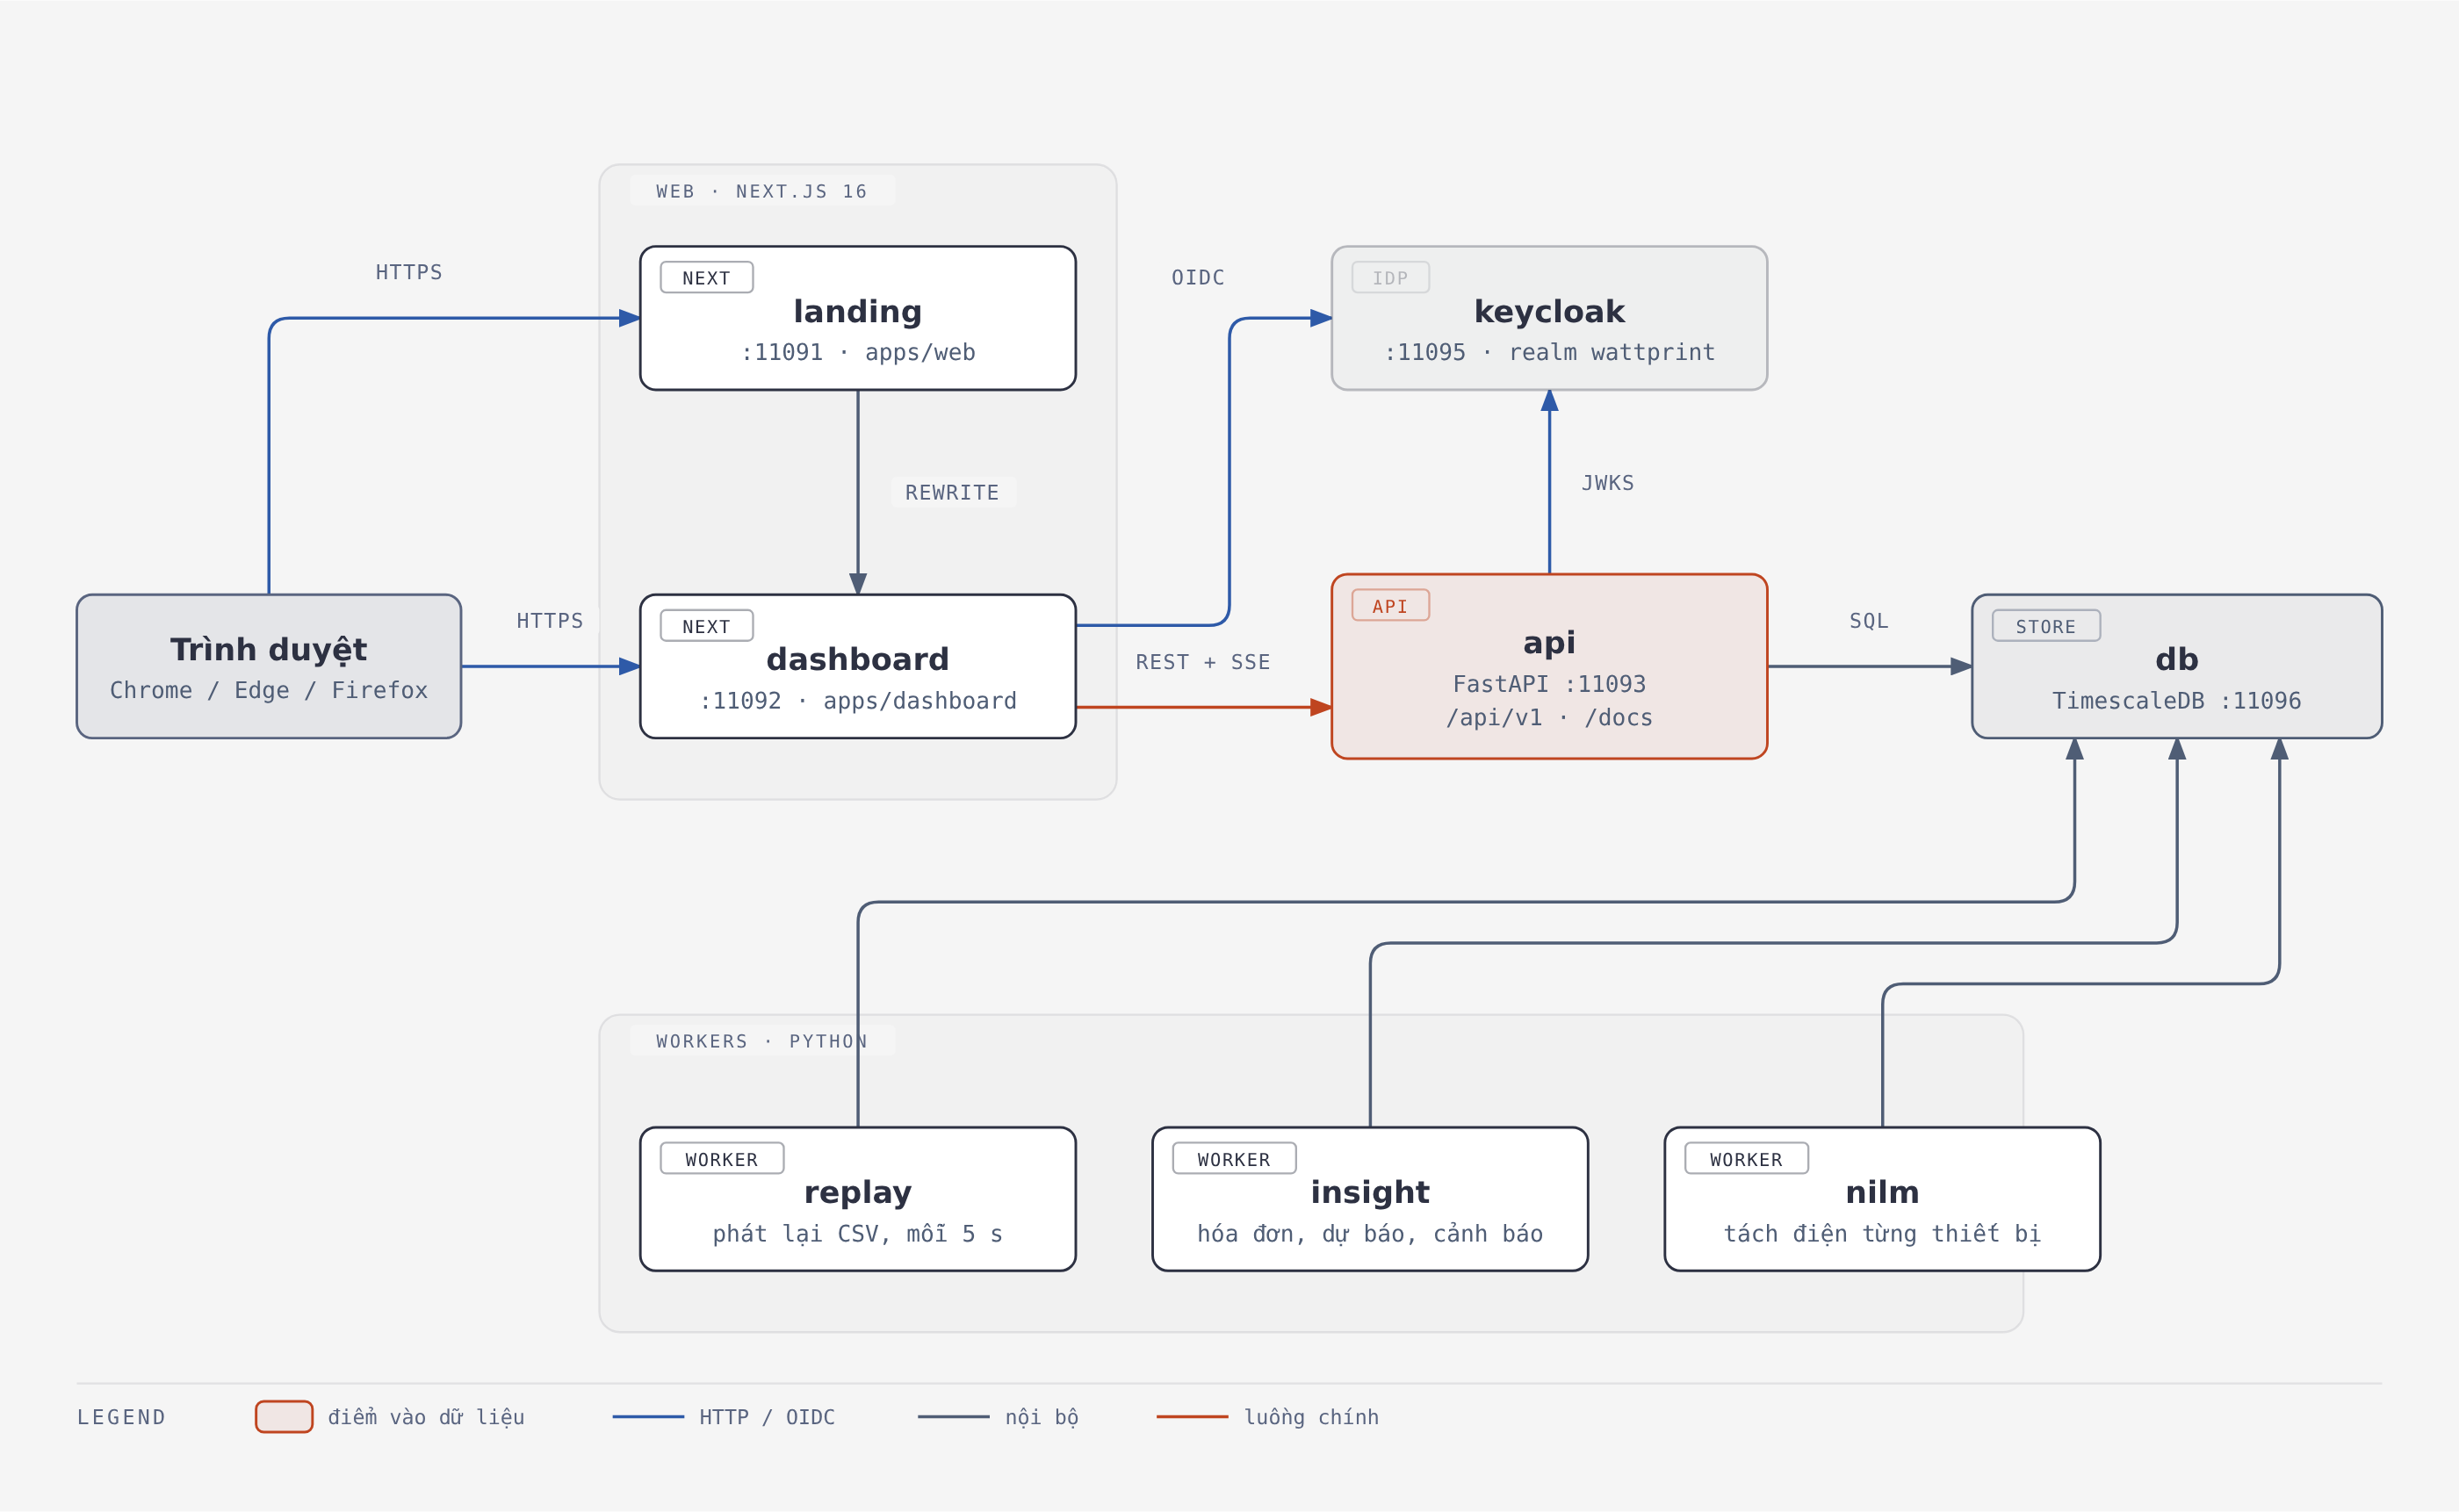
\includegraphics[width=.7\linewidth]{figures/dgt_be_system.png}\caption{Kiến trúc backend và web trong Docker Compose: 01 API, 03 worker, 01 cơ sở dữ liệu.}\label{fig:be}\end{figure}

\begin{figure}[H]\centering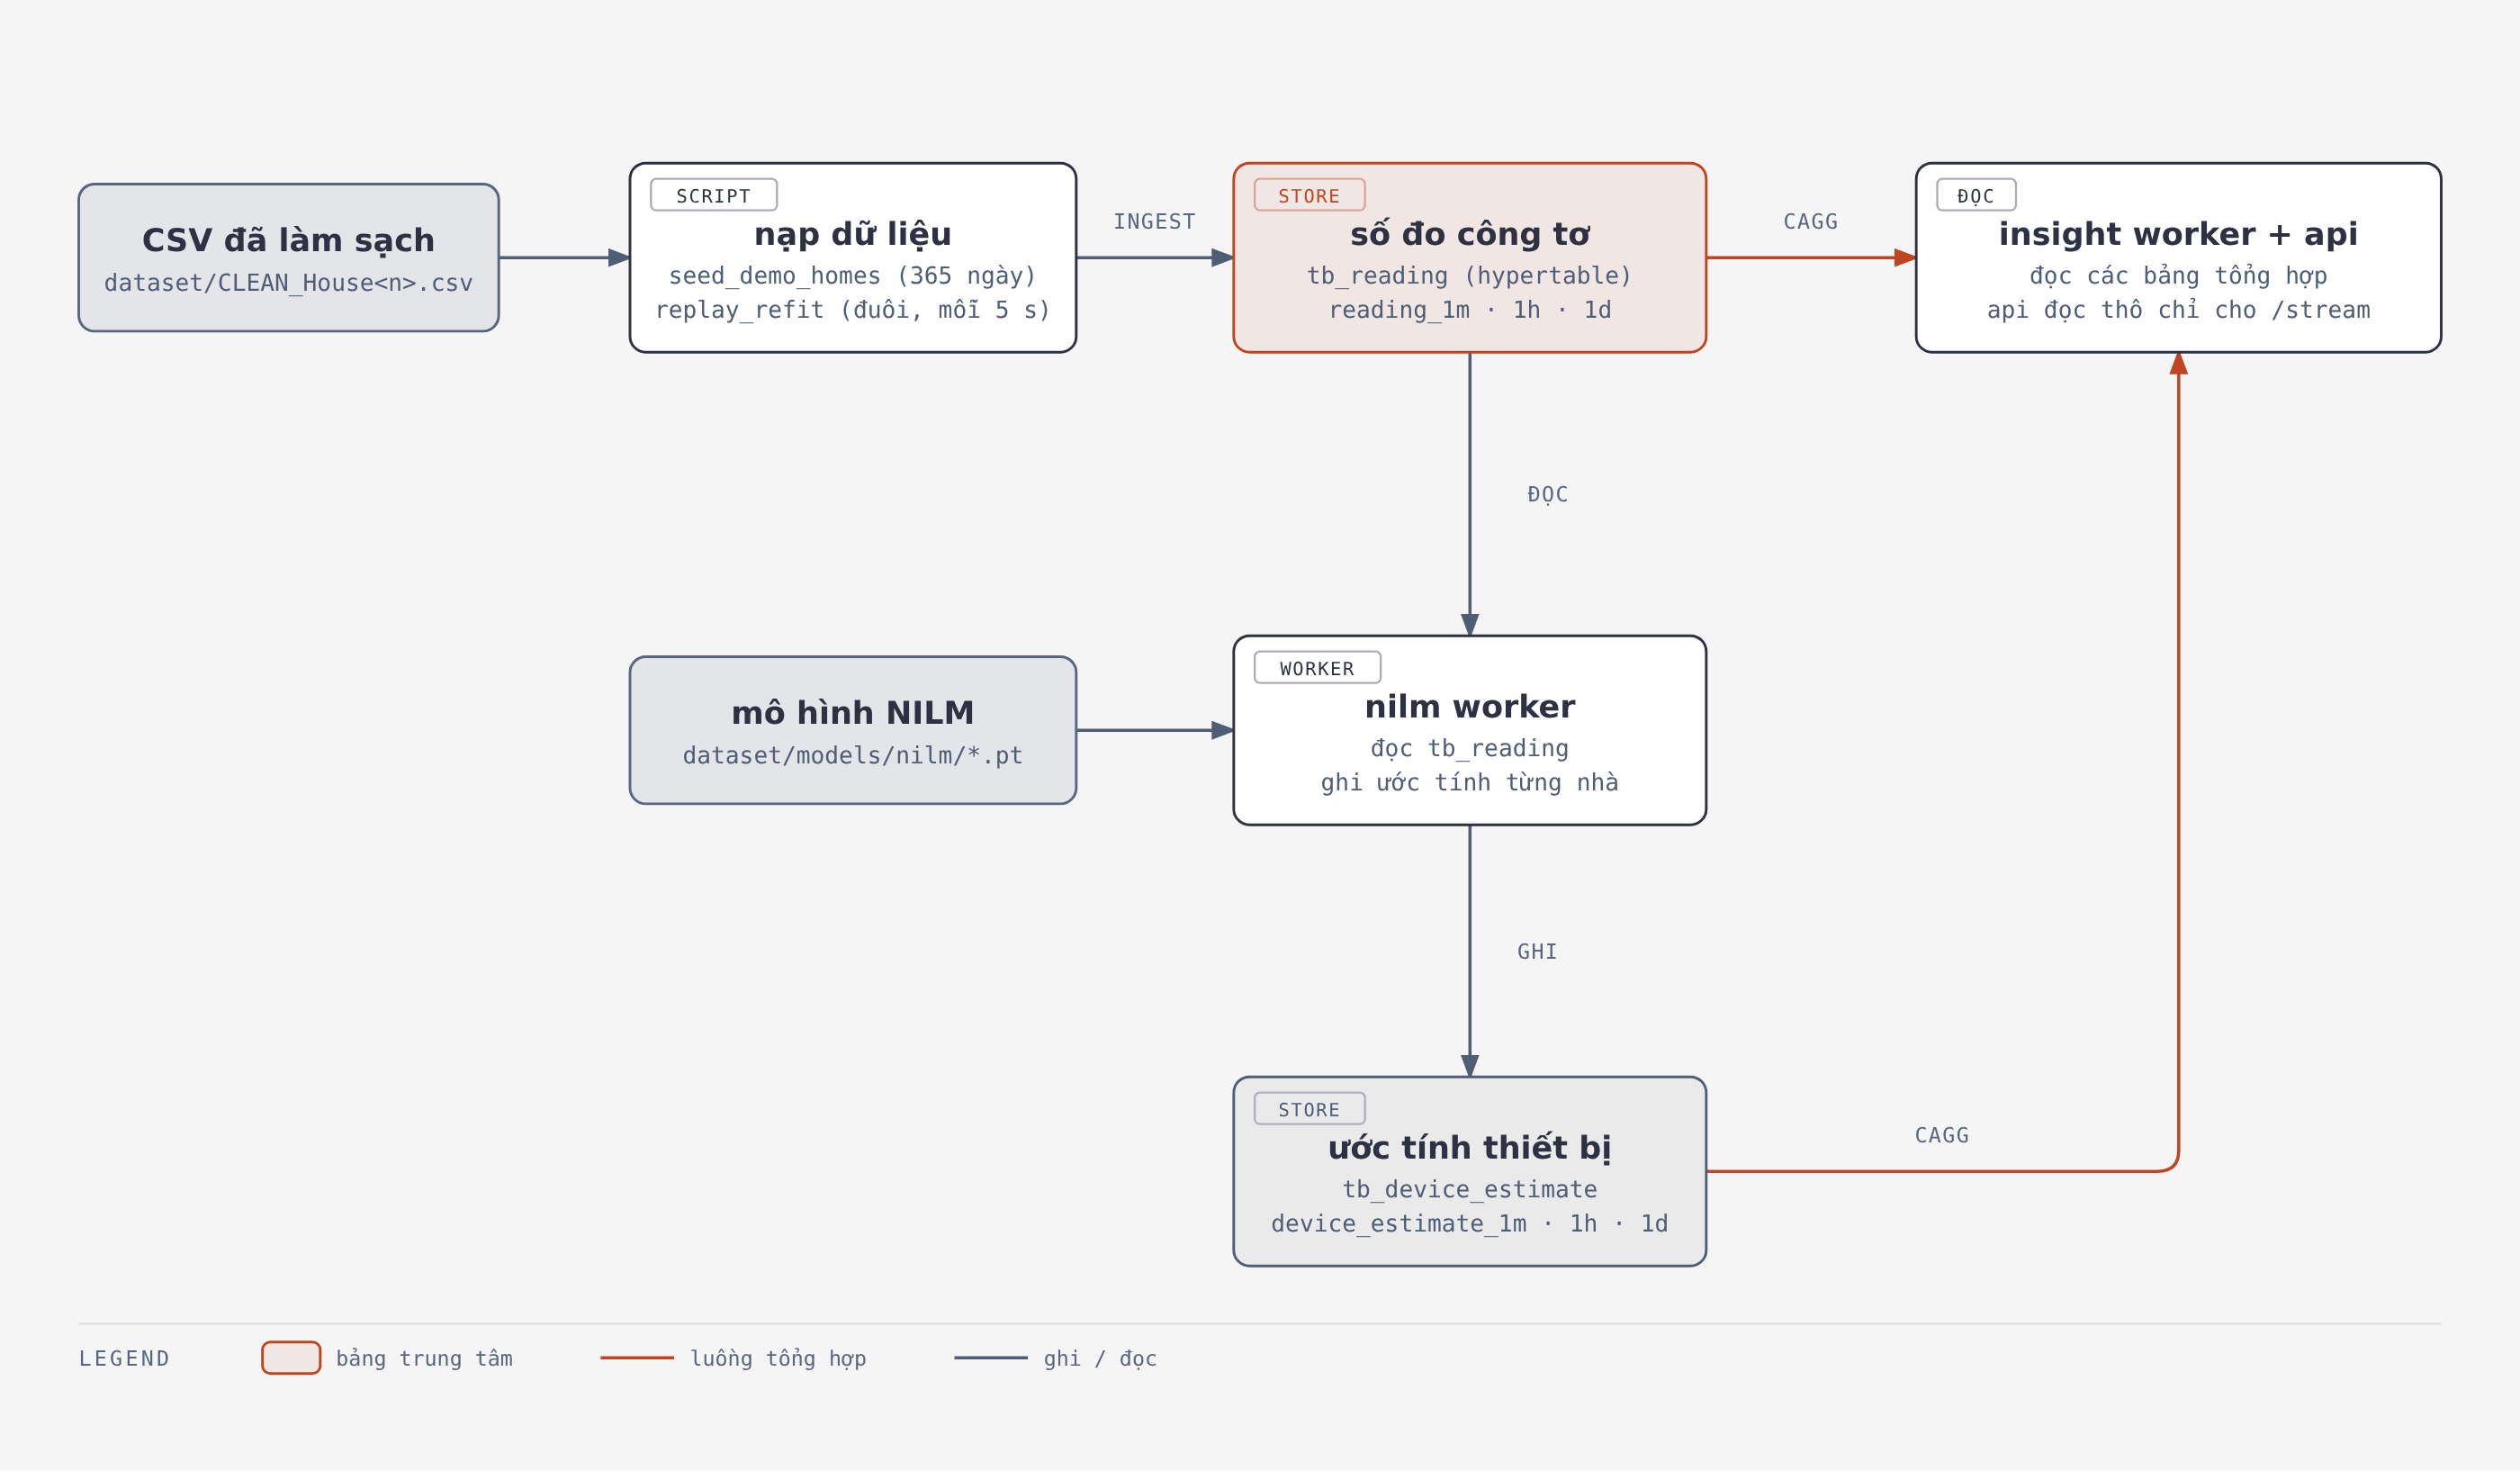
\includegraphics[width=.7\linewidth]{figures/dgt_be_reading.png}\caption{Đường đi của số đo điện: từ công tơ đến cơ sở dữ liệu, mô hình NILM và màn hình.}\label{fig:reading}\end{figure}

\paragraph*{Phân rã điện năng trong ứng dụng.}
Worker \texttt{nilm} đọc số đo tổng, chạy mô hình của từng nhà và ghi điện năng ước tính từng thiết bị. Mỗi nhà demo có 01 mô hình riêng. 04 nhà demo dùng dữ liệu của REFIT (nhà 2 và 5) \citep{murray2017}, Plegma (nhà 1) \citep{athanasoulias2023} và ENERTALK (nhà 0) \citep{shin2019}. Phần điện không gán được cho thiết bị nào hiện ở mục \emph{Khác}, kèm nhãn độ tin cậy Cao, Vừa hoặc Thấp. Kết quả ở mục~\ref{sec:nilm} cho thấy mô hình chung có F1 cao hơn trên đa số hộ. Mô hình riêng tốt hơn ở một số chỉ số năng lượng. Nhóm dự kiến thử mô hình chung trong ứng dụng ở bước tiếp theo và kiểm tra thêm sai số điện năng theo từng hộ.

\paragraph*{Wappi và text2sql.}
Wappi trả lời qua luồng SSE. Mọi con số đến từ 17 công cụ xác định, như hóa đơn, dự báo, so sánh kỳ, thời tiết và cảnh báo. Mô hình ngôn ngữ chỉ diễn giải kết quả của công cụ, không tự tính. Mỗi câu trả lời mang một mức nguồn gốc: đo trực tiếp, theo văn bản, ước tính hoặc suy luận. Với câu hỏi về luật và biểu giá, Wappi tìm kết hợp từ khóa và vector trong văn bản pháp luật đã nạp. Wappi ưu tiên văn bản mới nhất và nêu mã văn bản. Với câu hỏi dữ liệu tự do, Wappi gọi \texttt{text2sql}. Thành phần này dùng đồ thị LangGraph, tìm metric và cột liên quan trong Qdrant rồi sinh truy vấn SQL. Truy vấn chạy bằng một role chỉ đọc, chỉ thấy view của đúng một nhà. Dữ liệu cá nhân (email, số điện thoại, số tài khoản) bị che trước khi lưu hoặc gửi đi. Bộ lọc prompt injection chạy trước mô hình. Wappi hỗ trợ nhập bằng giọng nói và đọc to câu trả lời.

\begin{figure}[H]\centering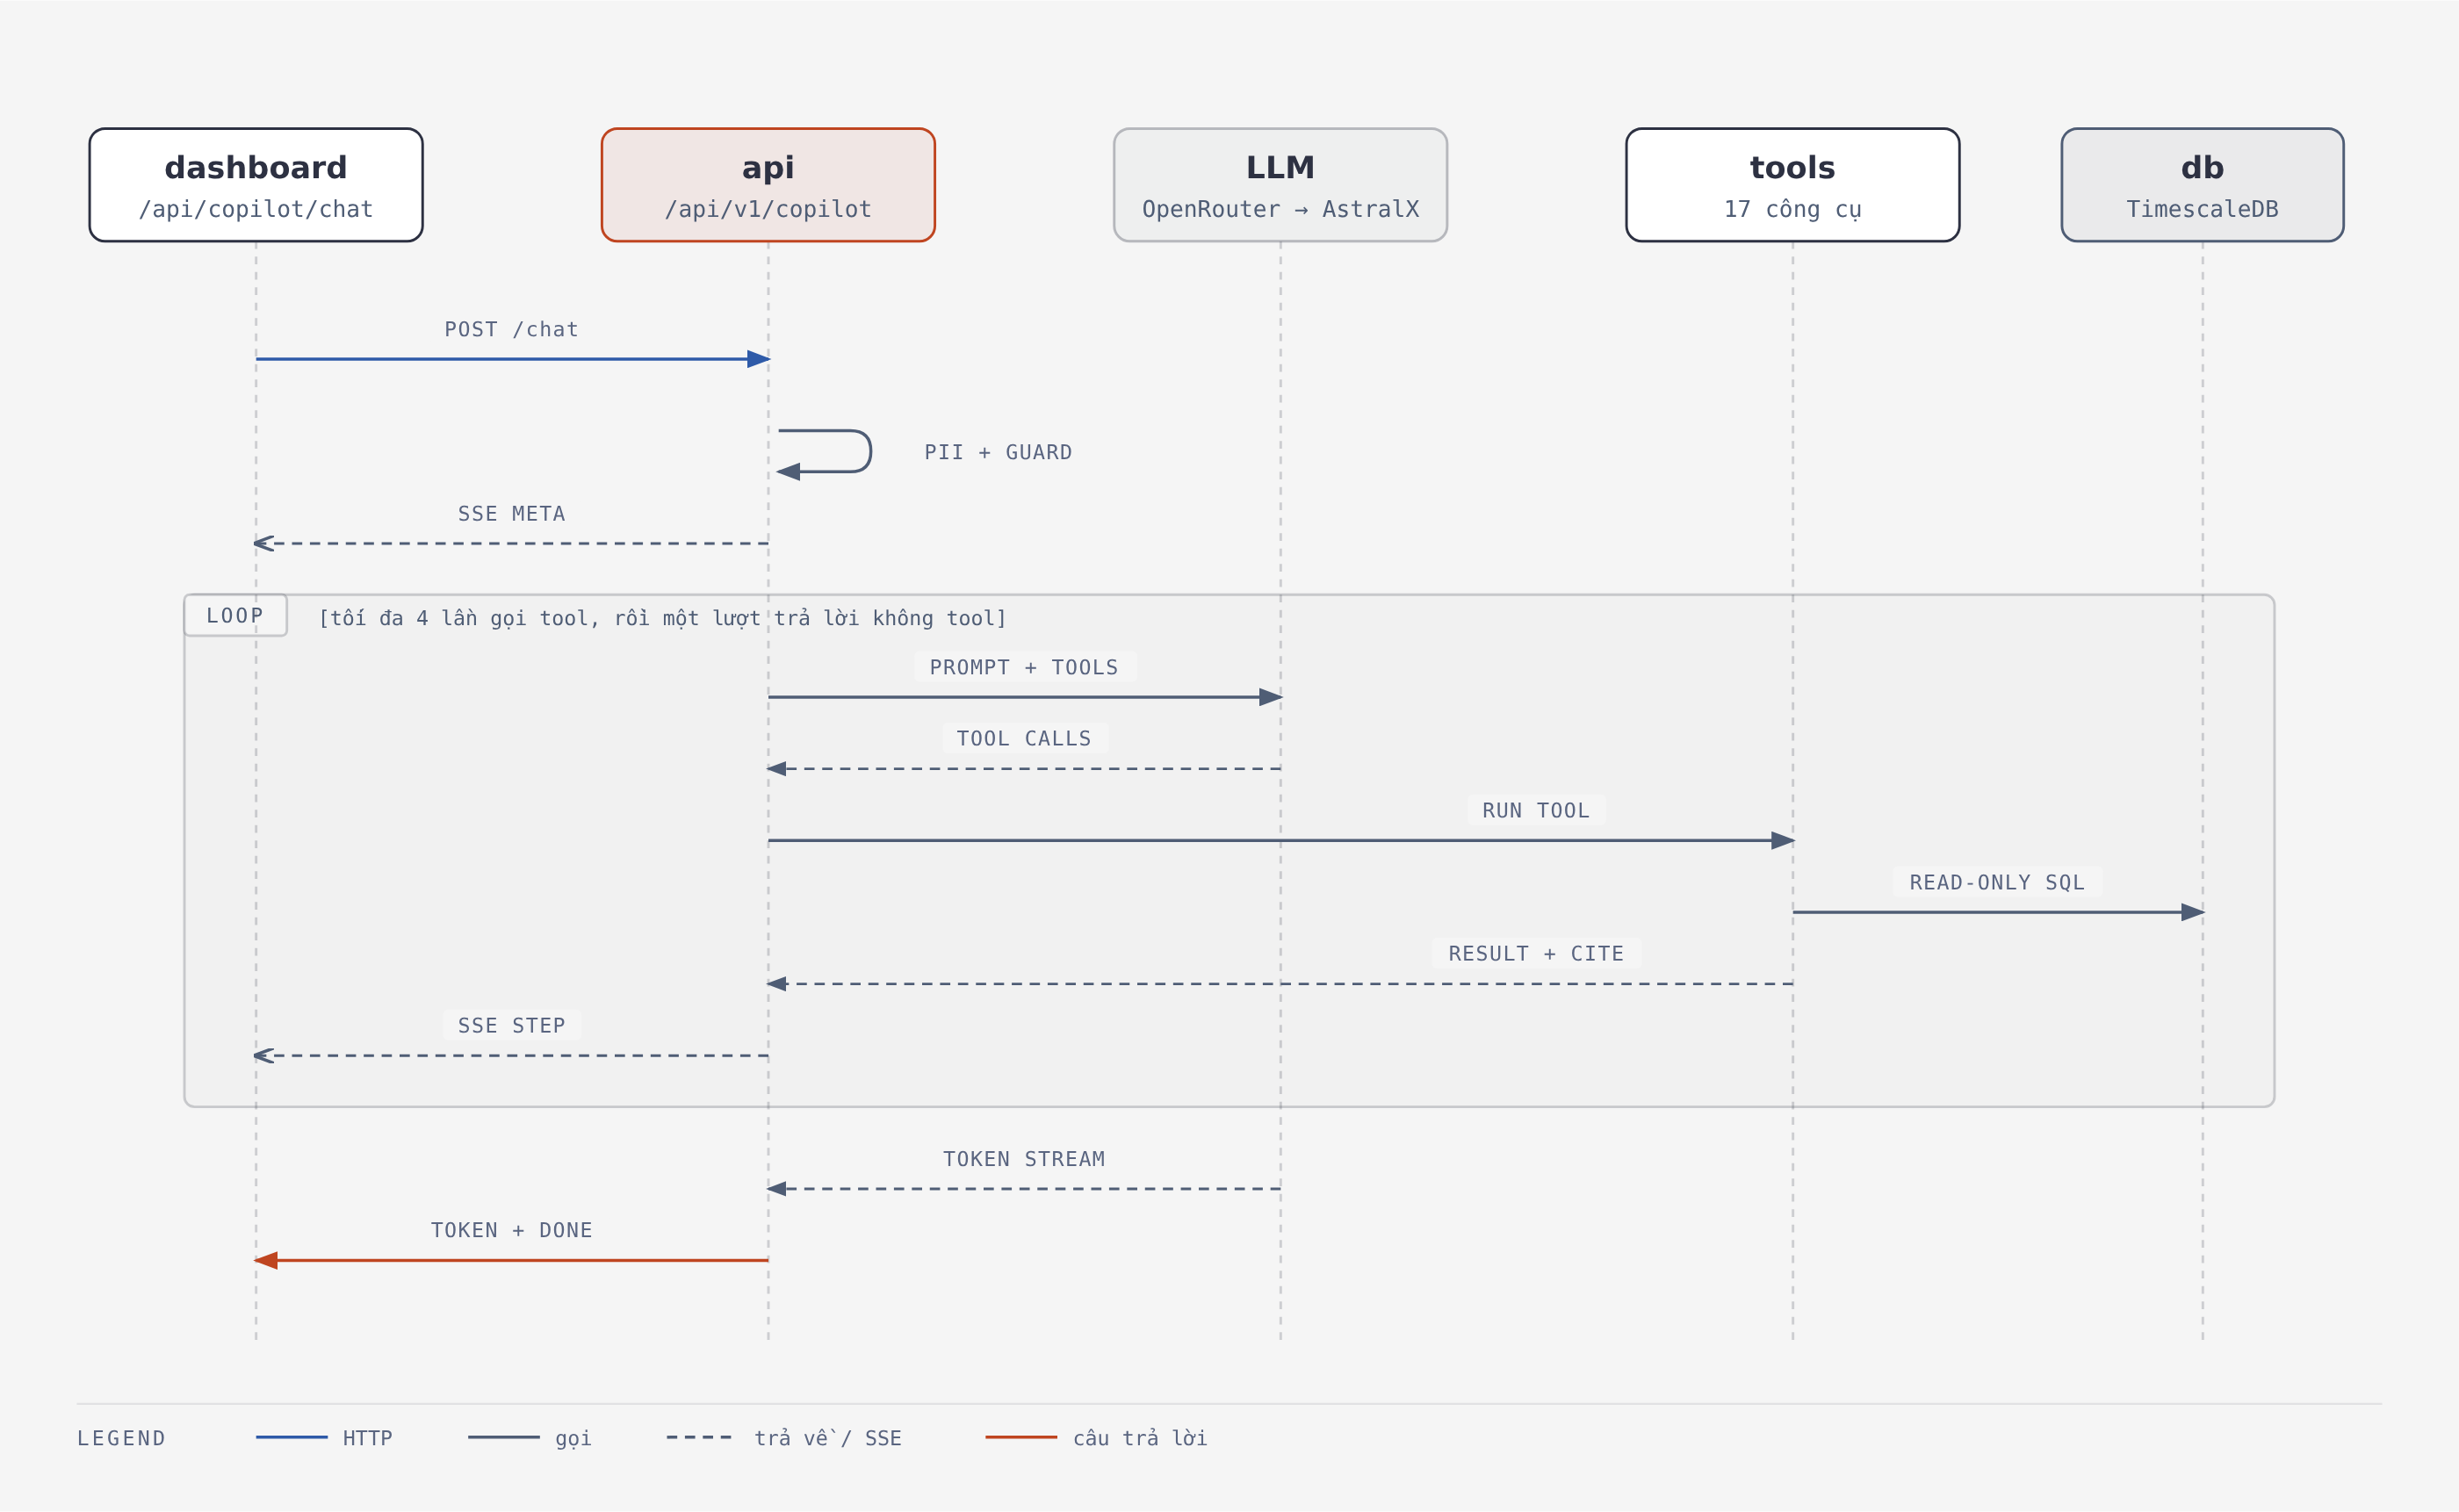
\includegraphics[width=.7\linewidth]{figures/dgt_be_wappi.png}\caption{Một lượt hỏi đáp với Wappi: công cụ tính số liệu, mô hình ngôn ngữ chỉ diễn giải.}\label{fig:wappichat}\end{figure}

\begin{figure}[H]\centering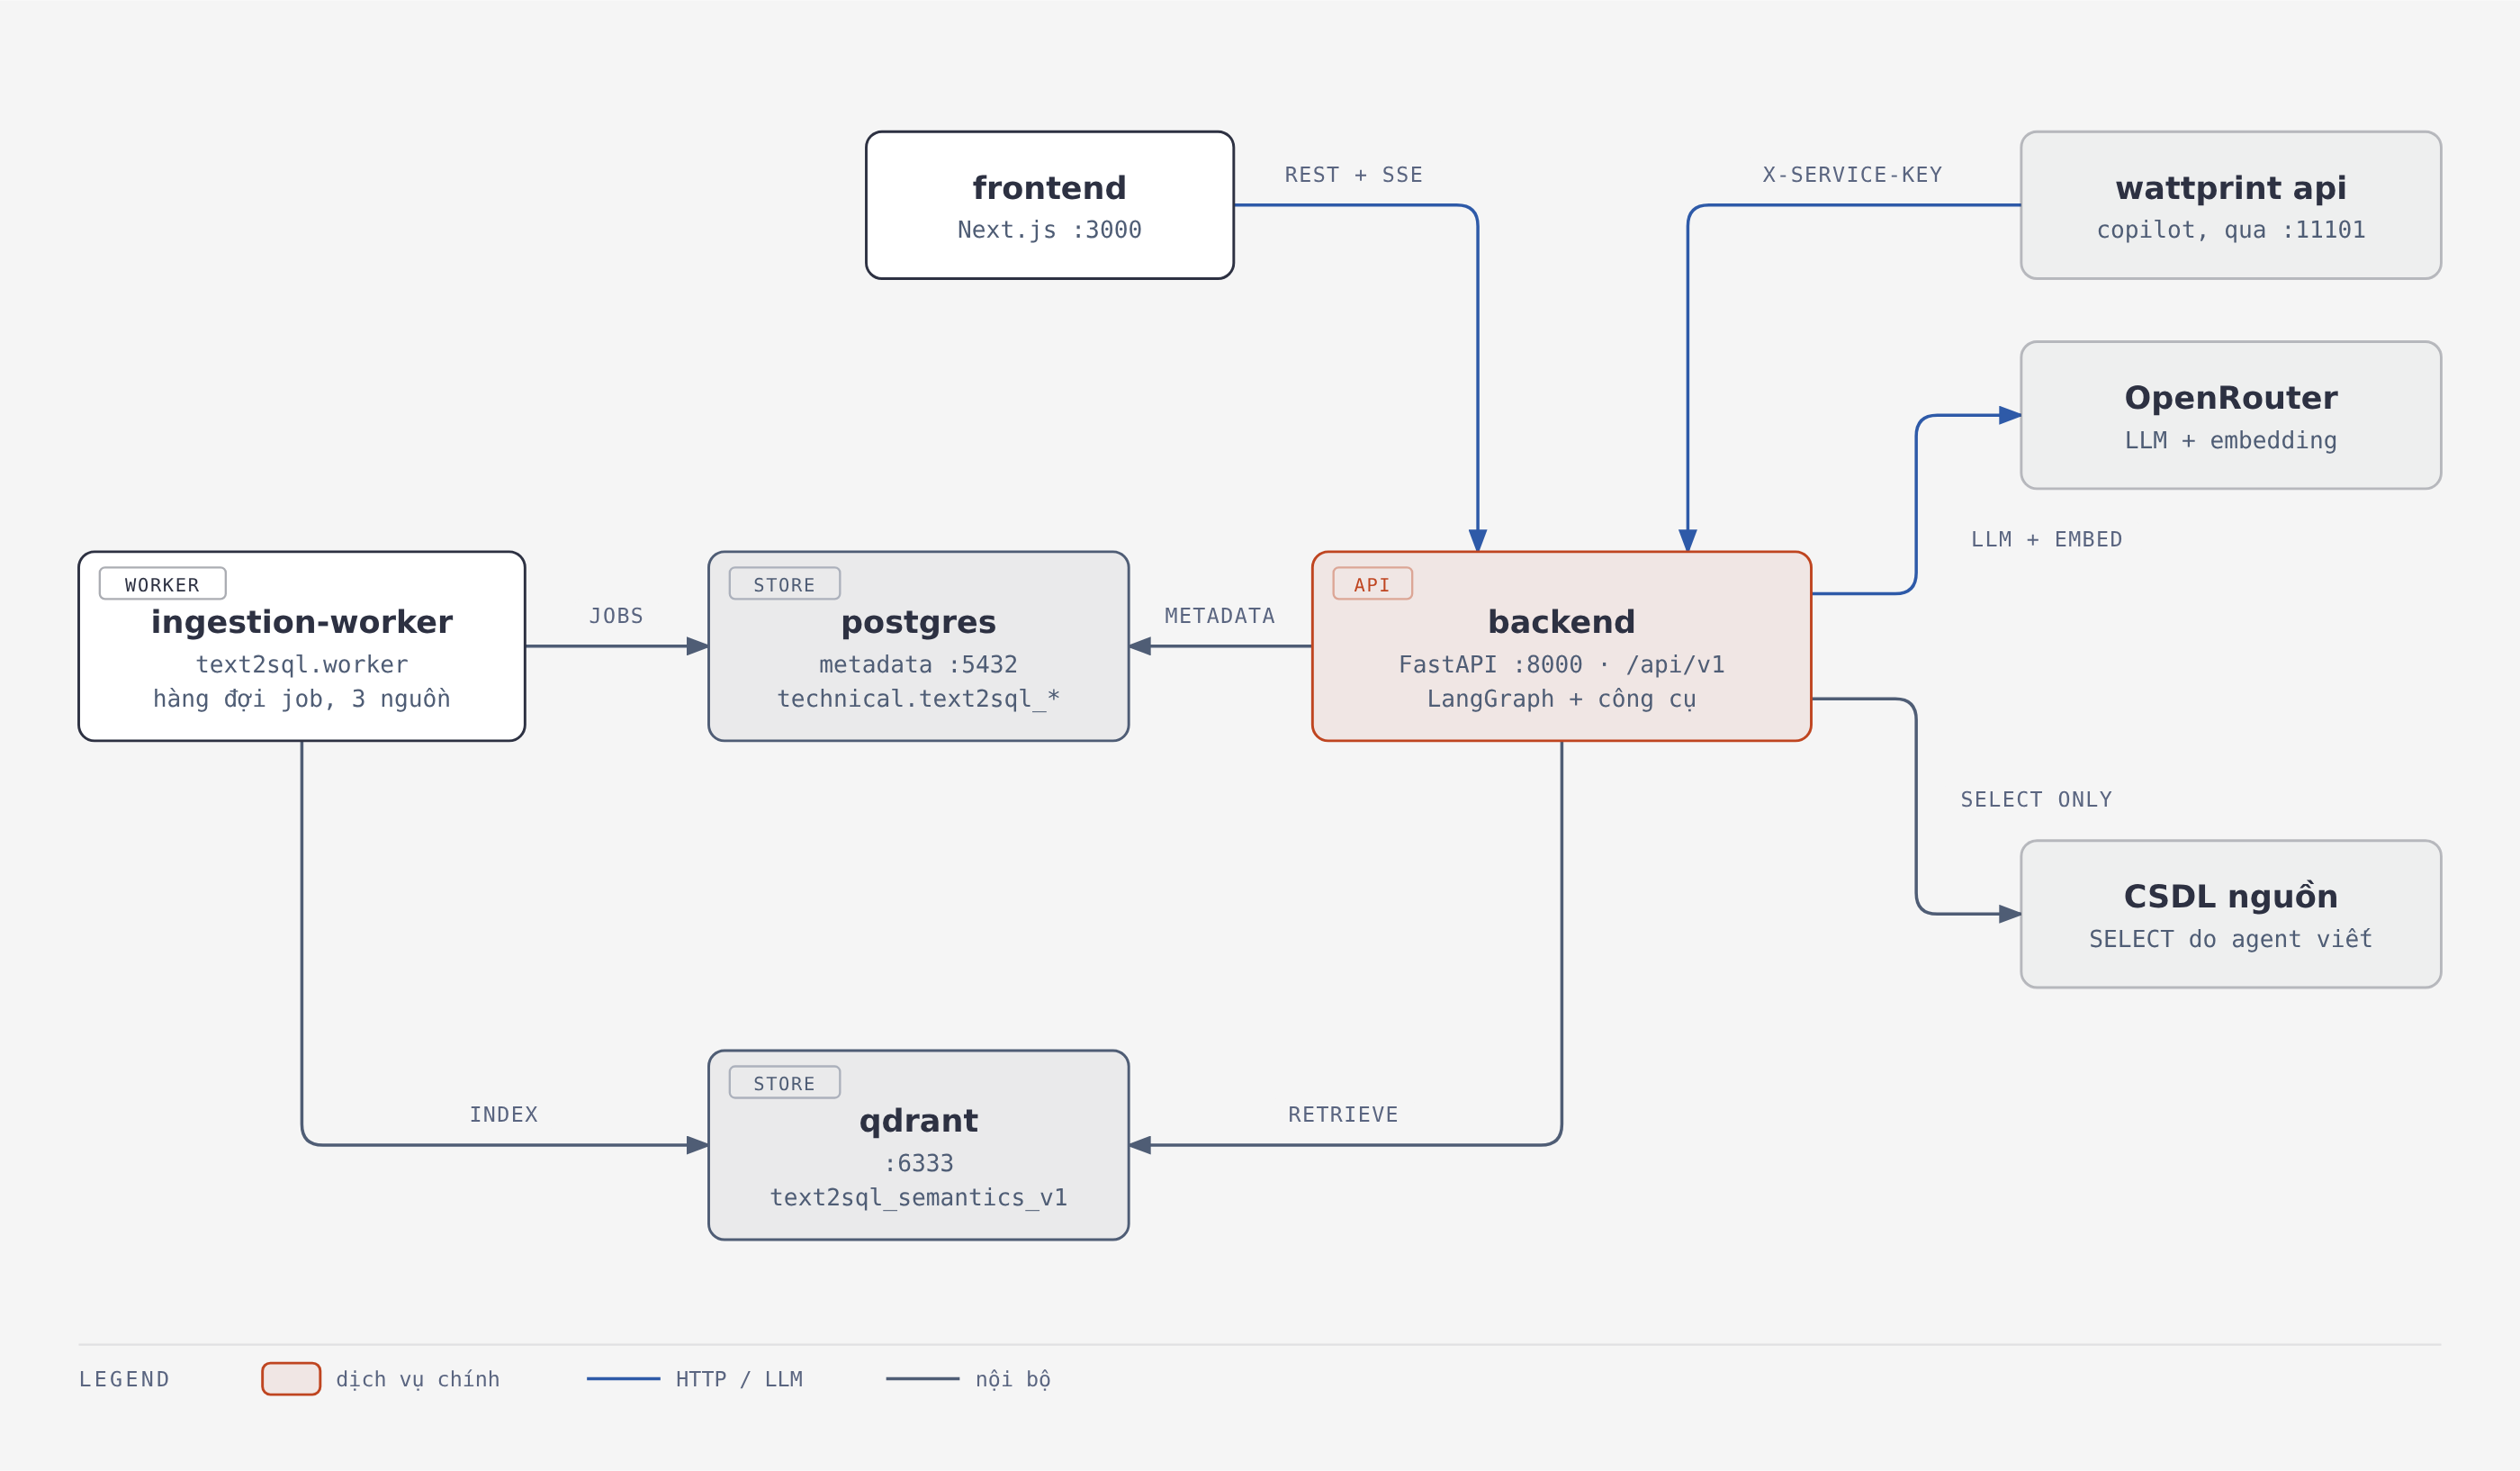
\includegraphics[width=.7\linewidth]{figures/dgt_t2s_arch.png}\caption{Kiến trúc thành phần text2sql của Wappi.}\label{fig:t2s}\end{figure}

\begin{figure}[H]\centering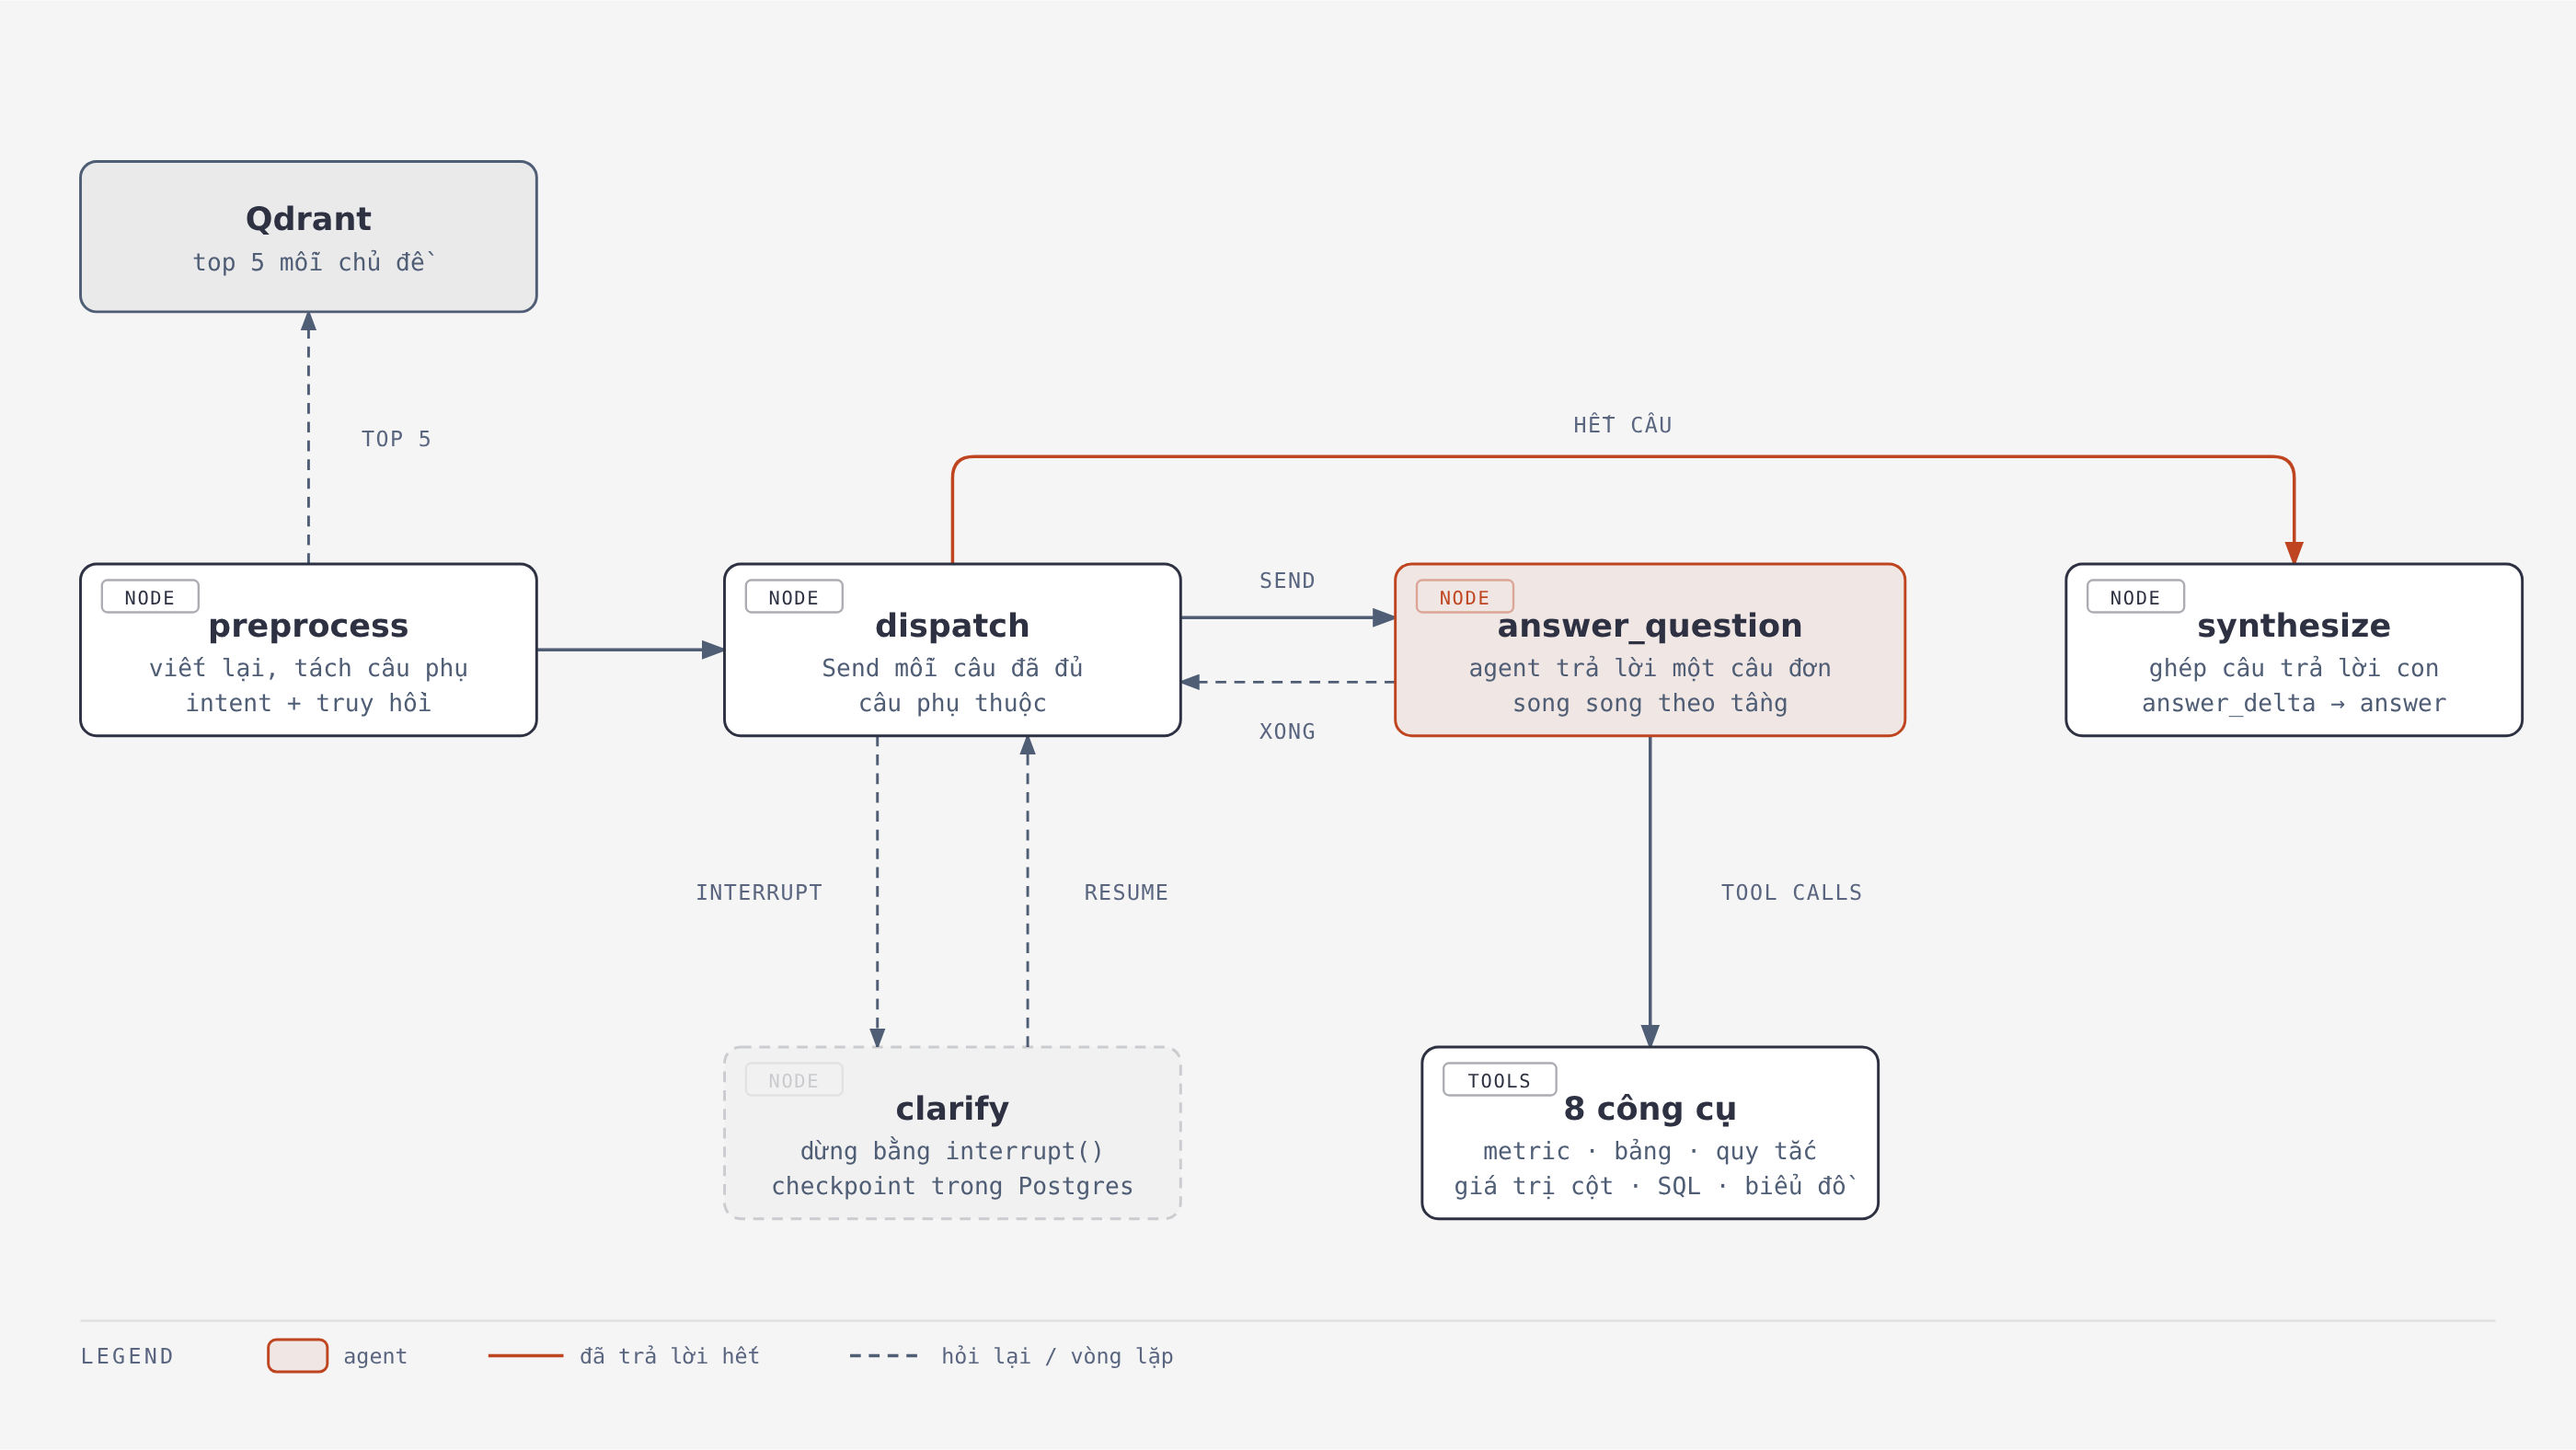
\includegraphics[width=.7\linewidth]{figures/dgt_t2s_chat.png}\caption{Đồ thị LangGraph của text2sql: từ câu hỏi đến truy vấn SQL chỉ đọc.}\label{fig:t2schat}\end{figure}

\paragraph*{Web.}
\texttt{apps/dashboard} và \texttt{apps/web} (trang giới thiệu) cùng một monorepo, dùng chung gói giao diện và gói xác thực. Token Keycloak nằm trong cookie \texttt{httpOnly} và không bao giờ tới trình duyệt. Dữ liệu từ API được kiểm bằng schema Zod trước khi hiển thị. Giao diện có tiếng Việt, tiếng Anh, chế độ sáng và tối. Người xem thử bấm \emph{Xem nhà demo} để vào ngay một nhà, không cần tài khoản. Tài khoản khách chỉ đọc và tự xóa sau khoảng 24 giờ.

\begin{figure}[H]\centering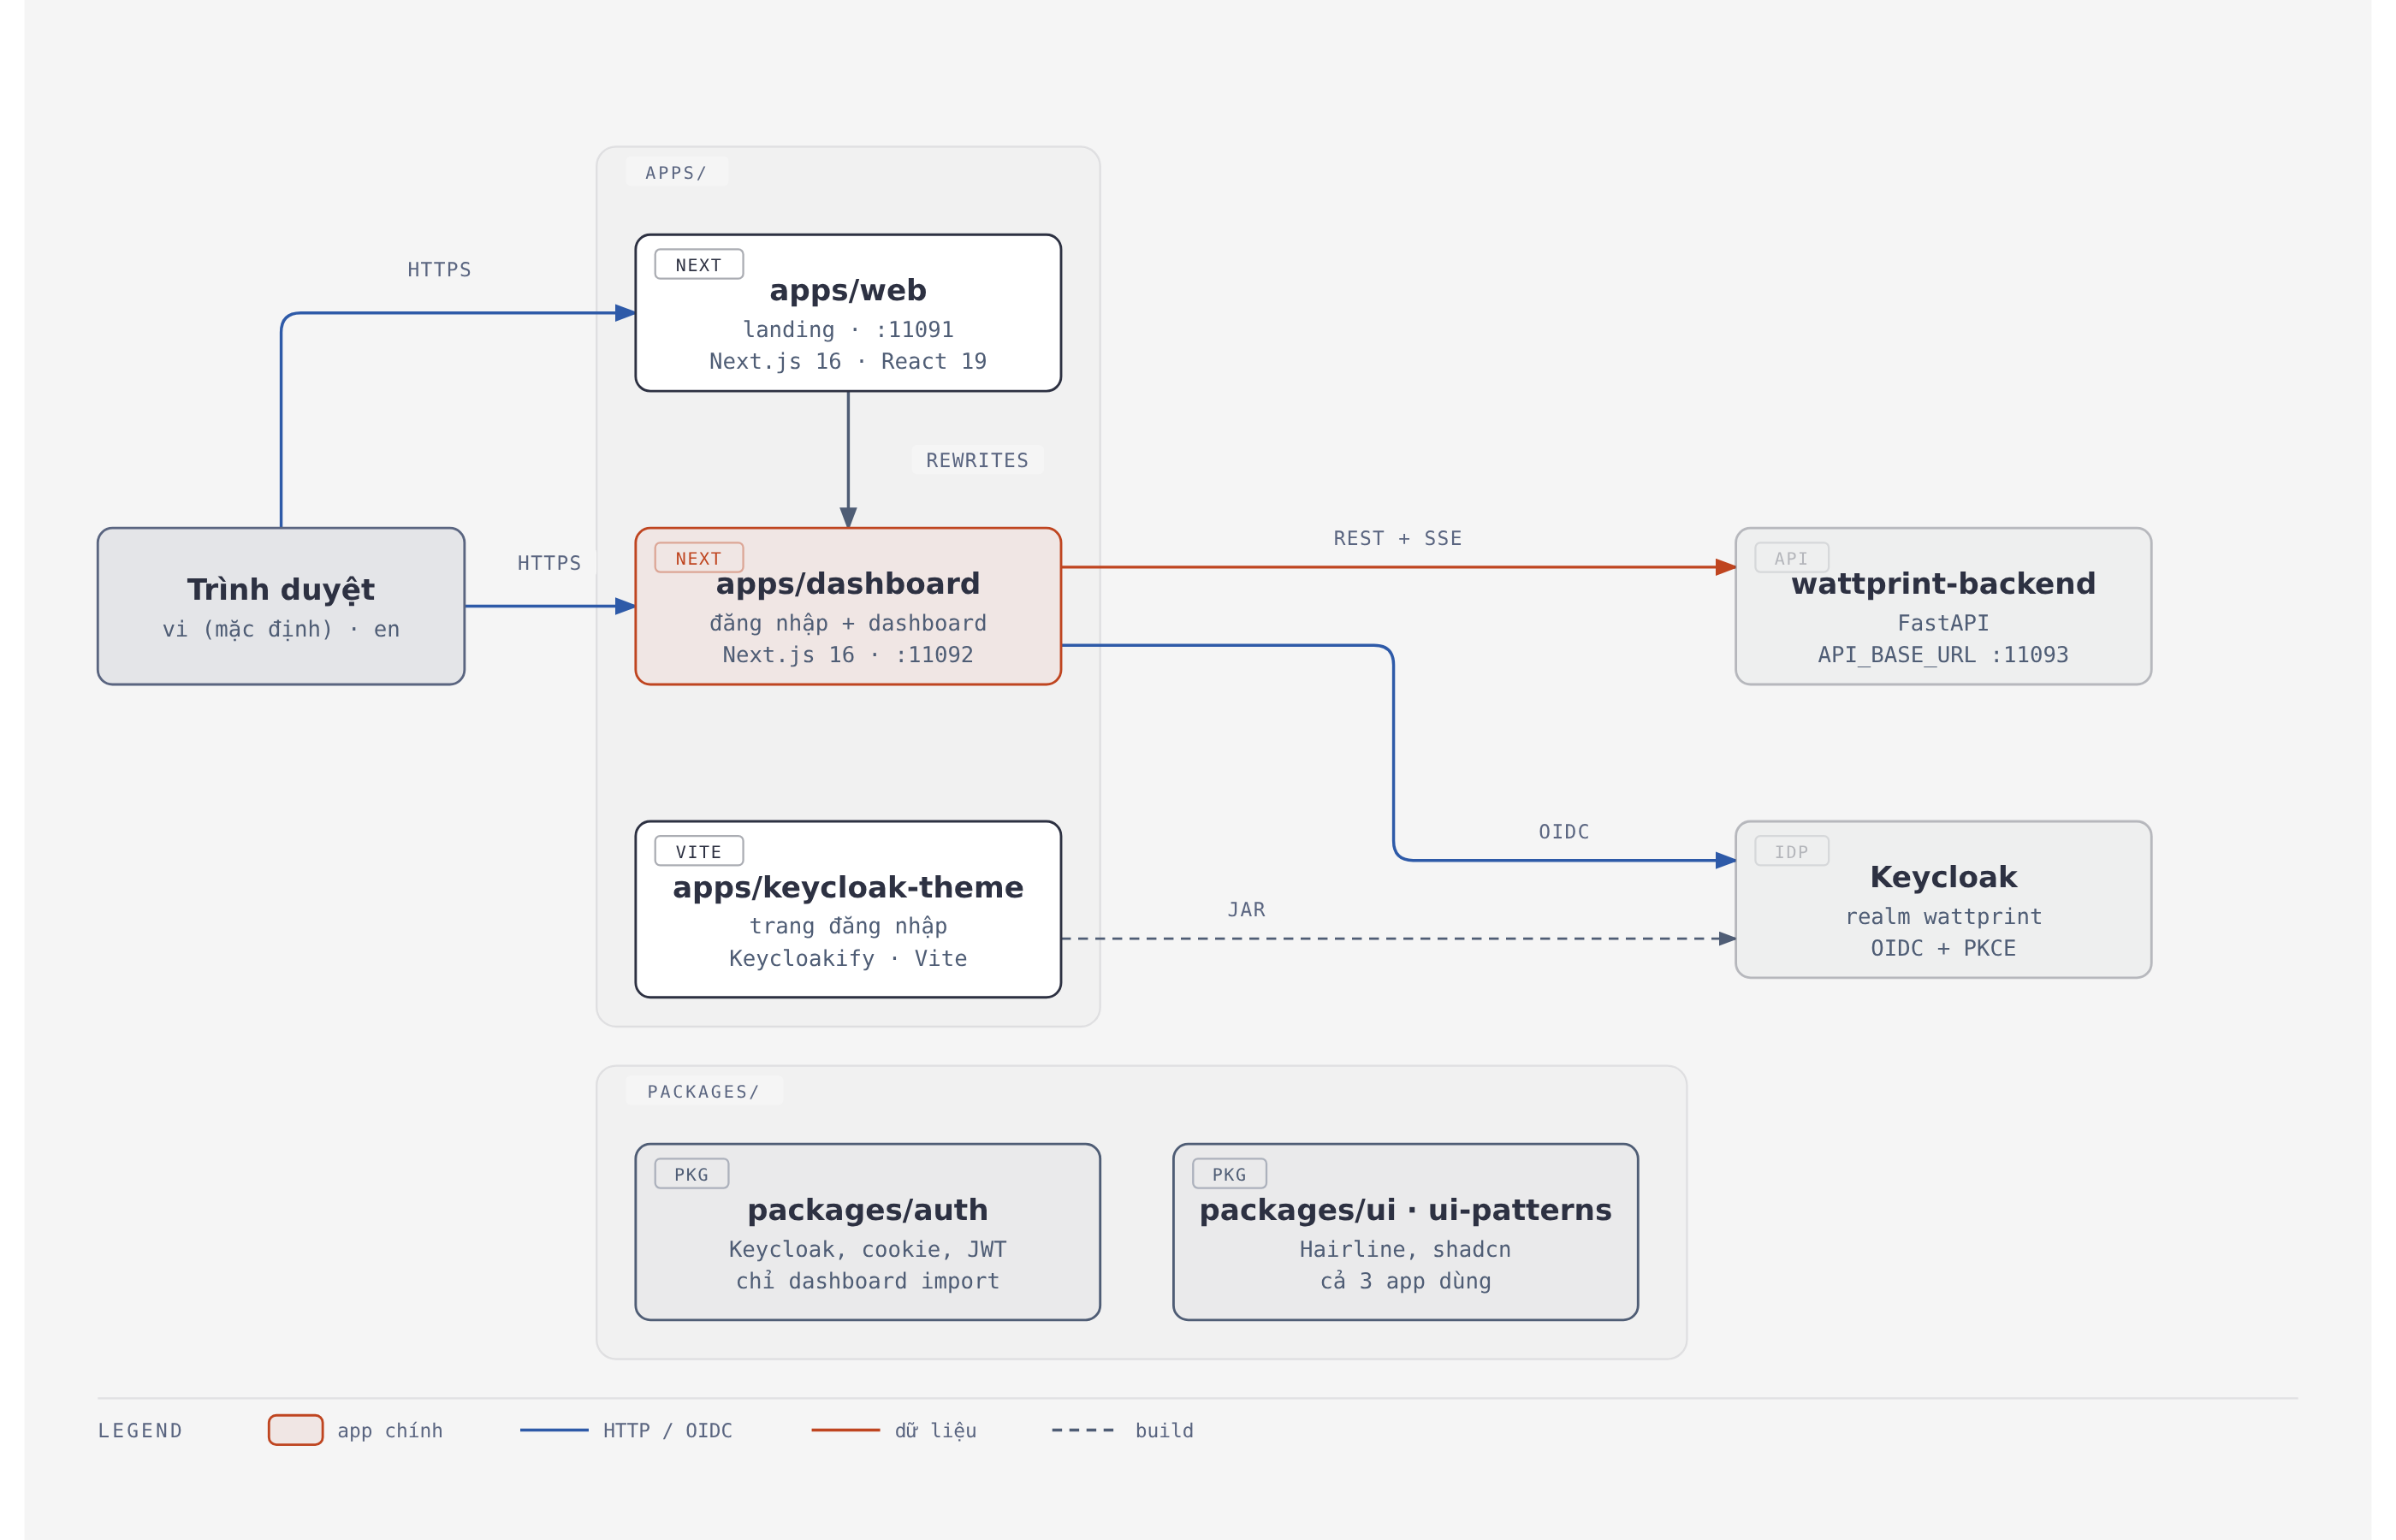
\includegraphics[width=.7\linewidth]{figures/dgt_web_arch.png}\caption{Kiến trúc monorepo web: 02 ứng dụng Next.js, giao diện đăng nhập Keycloak và các gói dùng chung.}\label{fig:webarch}\end{figure}

\paragraph*{nilm-eval.}
Project này chứa mã huấn luyện, mã đánh giá và phần đóng gói suy luận CPU bằng Docker. Kiến trúc mô hình 2Stage nằm ở Hình~\ref{nilm:fig2}.

\subsection{Chức năng đã hoàn thiện trên web}

Hình~\ref{fig:w1}, \ref{fig:w2} và \ref{fig:w4} là ảnh chụp toàn trang từ hệ thống đang chạy, nhà REFIT House 2.

\begin{itemize}
\item \textbf{Tổng quan.} Điện từng thiết bị, kèm nhãn \emph{Ước tính, tin cậy thấp} khi phần \emph{Khác} chiếm 77\%. Hóa đơn kỳ này theo bậc giá và số kWh còn lại của bậc hiện tại. Cảnh báo cần xem và nhật ký thiết bị 24 giờ.
\item \textbf{Thống kê.} Tiền điện kỳ này theo thiết bị và dự báo hóa đơn cuối kỳ. Công suất cả nhà theo 24 giờ, 7, 30 hoặc 90 ngày, so với mức thường lệ.
\item \textbf{Thiết bị.} Trạng thái bật hoặc tắt, công suất hiện tại, điện hôm nay và tiền tháng này của từng thiết bị, kèm trang chi tiết.
\item \textbf{Cảnh báo.} Các loại tự động gồm điện nền ban đêm tăng, thiết bị chạy vào giờ hiếm thấy, dùng điện khác thường và sắp sang bậc giá mới. Người dùng bật hoặc tắt từng loại, hoặc nhờ Wappi theo dõi điều mình muốn.
\item \textbf{Kế hoạch tiết kiệm.} Người dùng chọn từ 01 đến 03 việc. Hệ thống tính số tiền tiết kiệm đến cuối kỳ theo bậc giá, rồi theo dõi kết quả đến hết kỳ.
\item \textbf{Hóa đơn.} Hóa đơn kỳ này, dự kiến cuối kỳ so với kỳ trước, giá và điện đã dùng ở từng bậc, hóa đơn các kỳ trước. Khi công tơ thiếu số đo, giao diện ghi rõ tiền điện có thể thấp hơn thực tế.
\item \textbf{Wappi.} Hỏi bằng chữ, nhập bằng giọng nói hoặc trò chuyện hoàn toàn bằng giọng nói. Câu trả lời kèm nguồn, thẻ số liệu, nút nghe và gợi ý hỏi tiếp (Hình~\ref{fig:w4}).
\end{itemize}

\newcommand{\cotanh}[3]{\begin{minipage}[t]{#1}\centering\includegraphics[width=\linewidth]{figures/#2.png}\\[1pt]{\footnotesize #3}\end{minipage}}
\begin{figure}[H]\centering
\cotanh{9.3cm}{p_tong_quan}{(a) Tổng quan}\hfill\cotanh{6.2cm}{p_thong_ke}{(b) Thống kê}
\caption{Trang Tổng quan và trang Thống kê, chụp toàn trang.}\label{fig:w1}
\end{figure}
\begin{figure}[H]\centering
\cotanh{7.6cm}{p_hoa_don}{(a) Hóa đơn}\hfill\cotanh{7.6cm}{p_canh_bao}{(b) Cảnh báo}\\[6pt]
\cotanh{7.6cm}{p_thiet_bi}{(c) Thiết bị}\hfill\cotanh{7.6cm}{p_ke_hoach}{(d) Kế hoạch tiết kiệm}
\caption{Trang Hóa đơn, Cảnh báo, Thiết bị và Kế hoạch tiết kiệm, chụp toàn trang.}\label{fig:w2}
\end{figure}
\begin{figure}[H]\centering
\setlength{\tabcolsep}{4pt}
\begin{tabular}{cc}
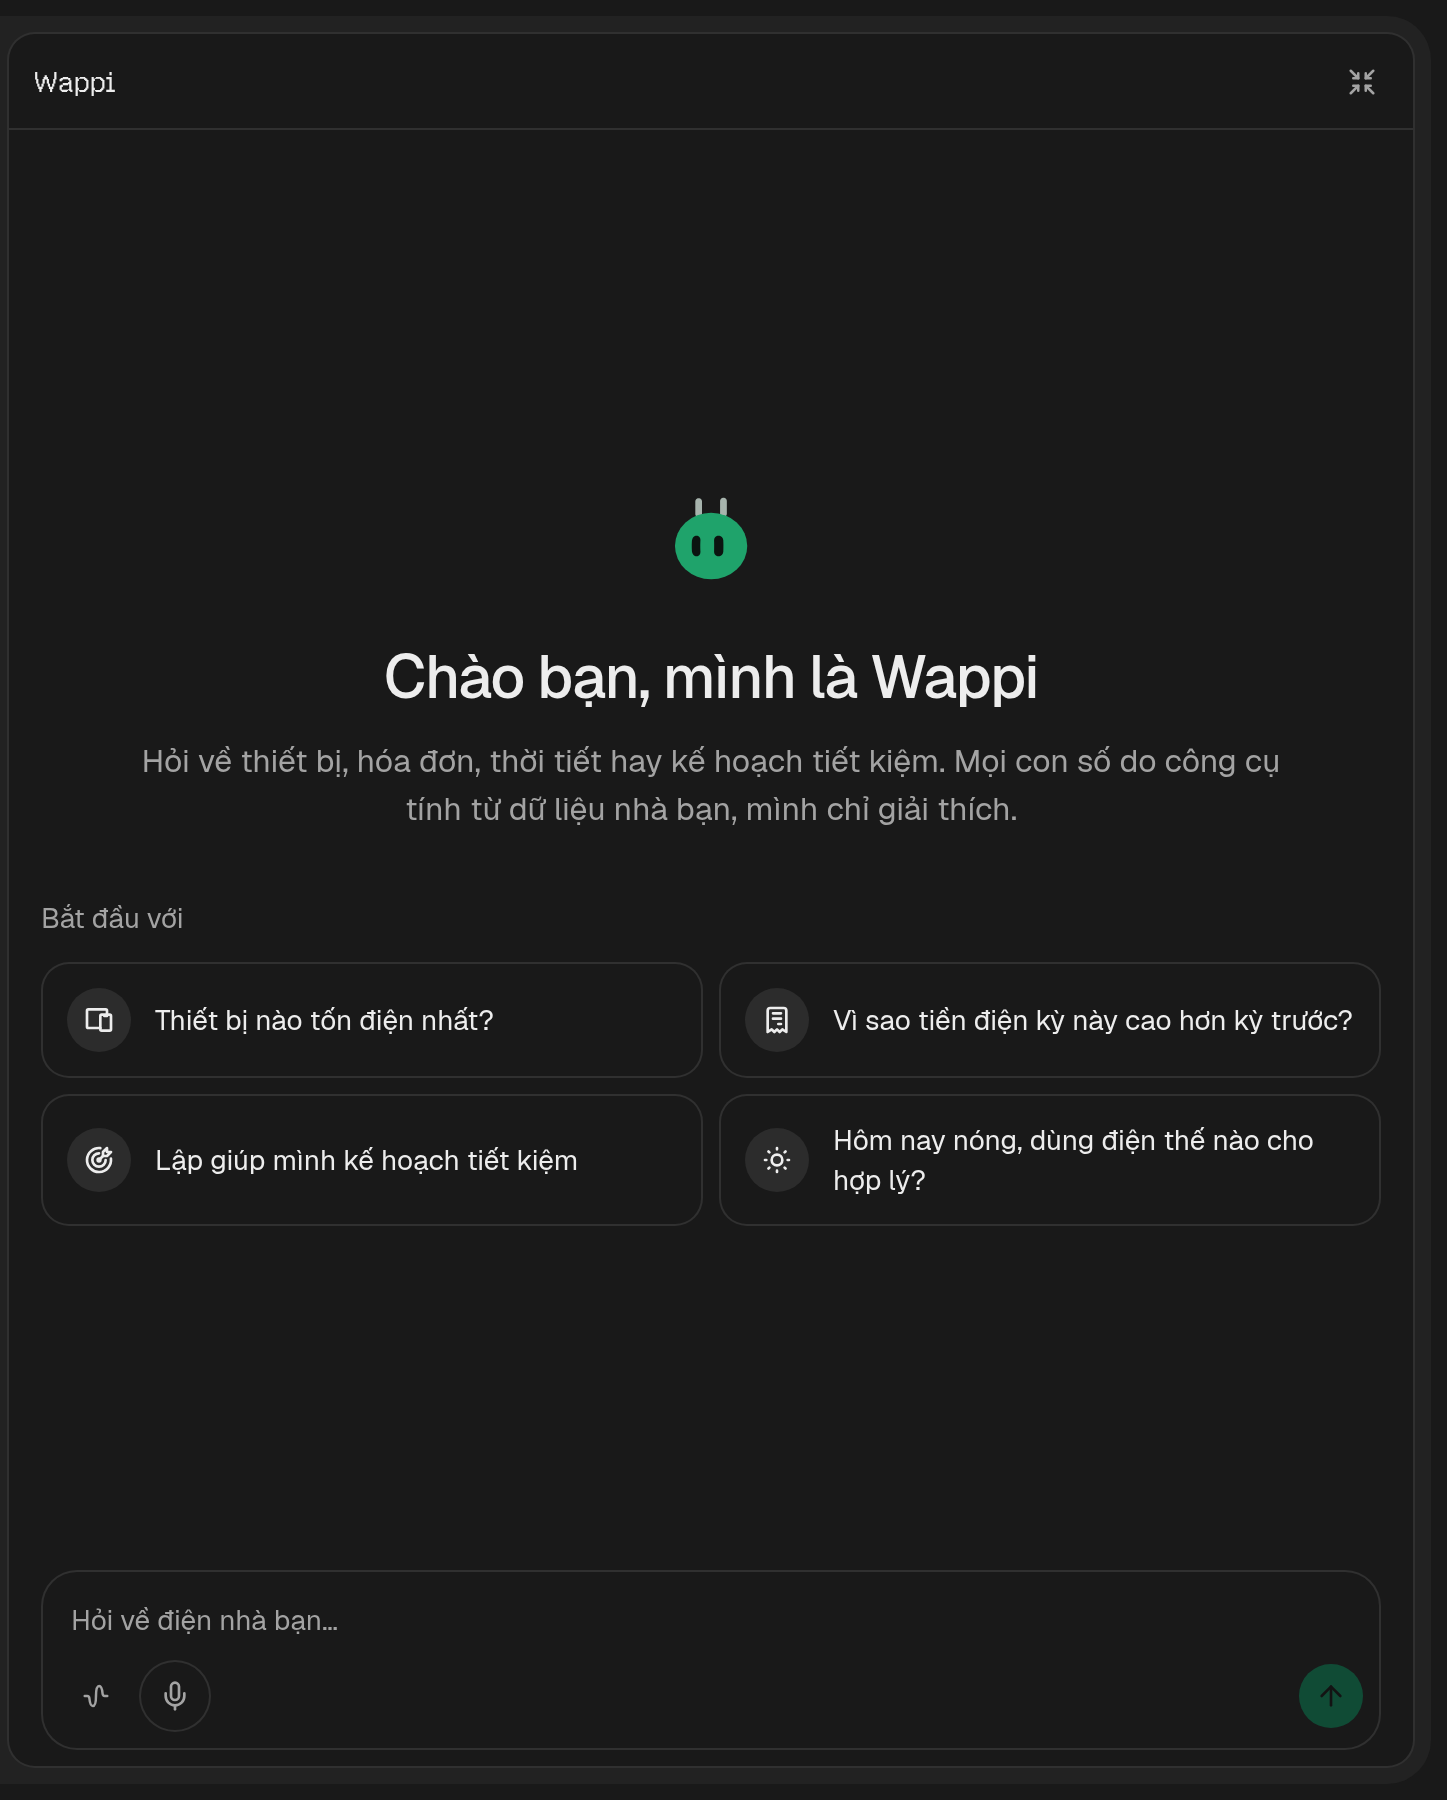
\includegraphics[height=6.6cm]{figures/q_a.png} & 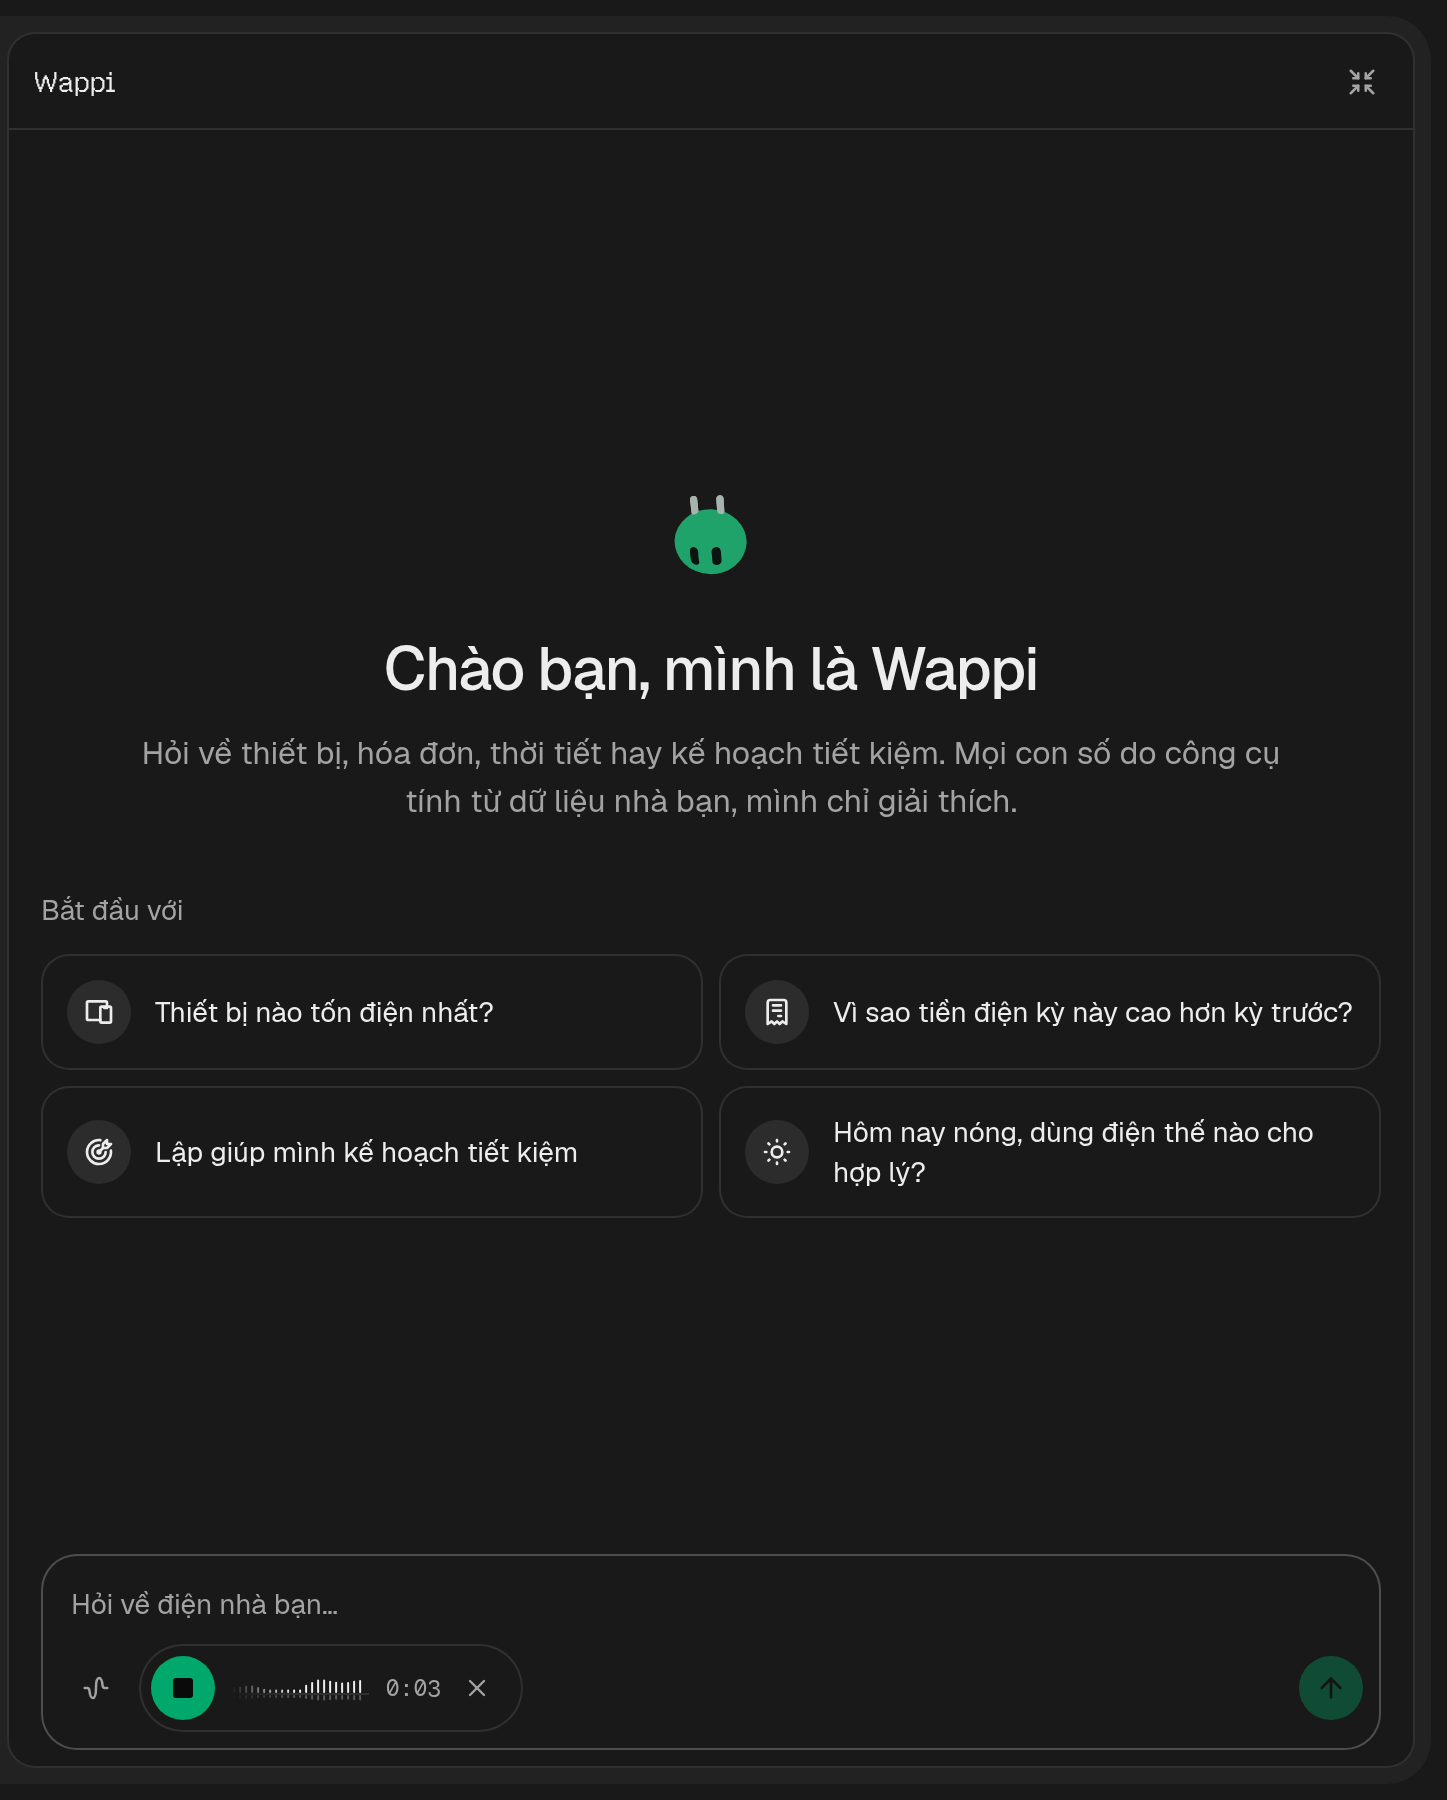
\includegraphics[height=6.6cm]{figures/q_b.png}\\
\small (a) Lúc mới vào & \small (b) Nhập bằng giọng nói, đang ghi âm\\[6pt]
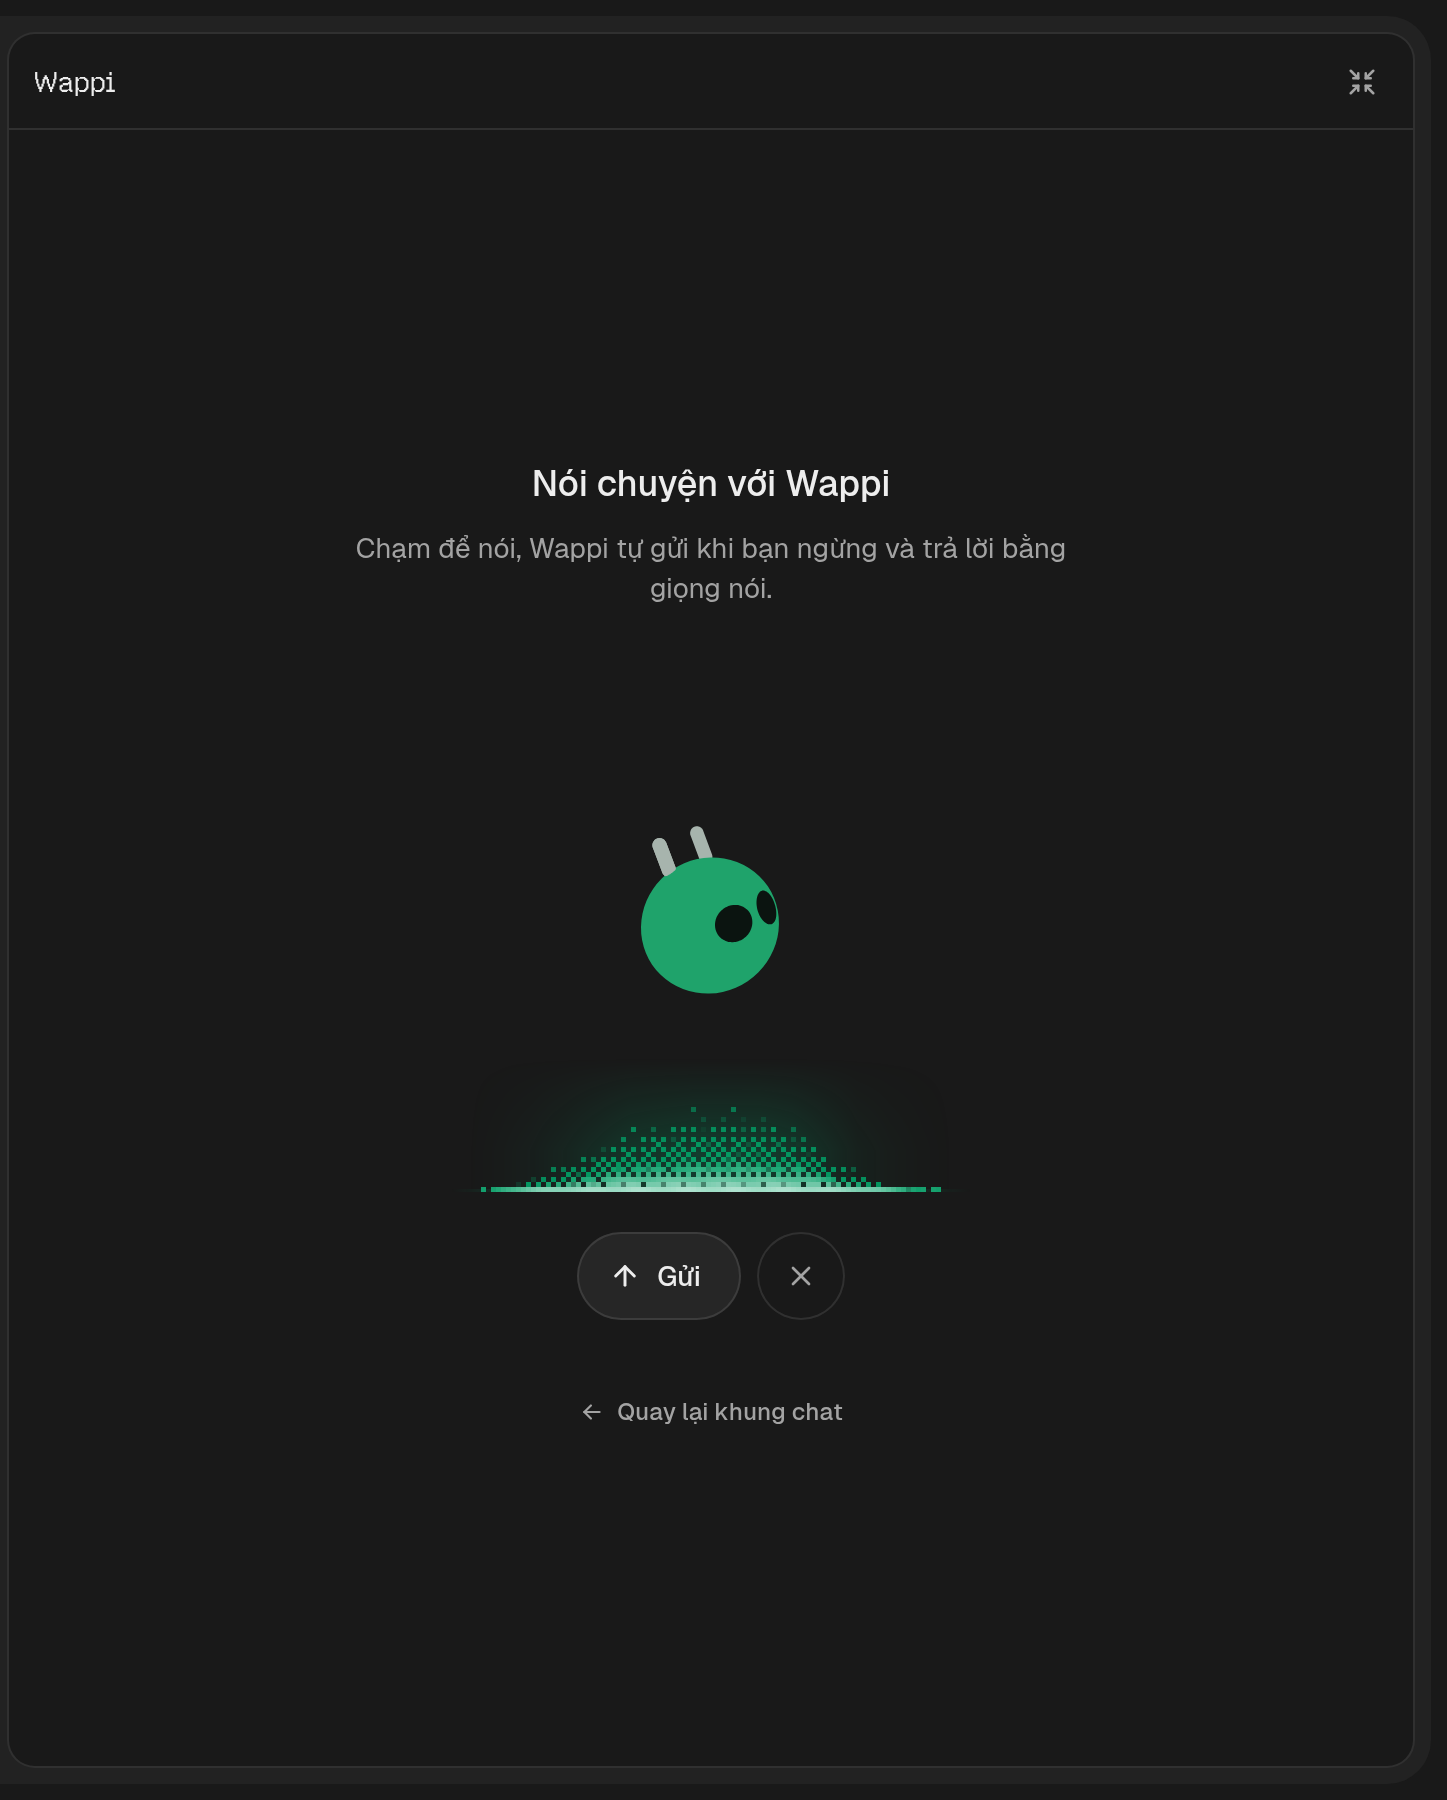
\includegraphics[height=6.6cm]{figures/q_c.png} & 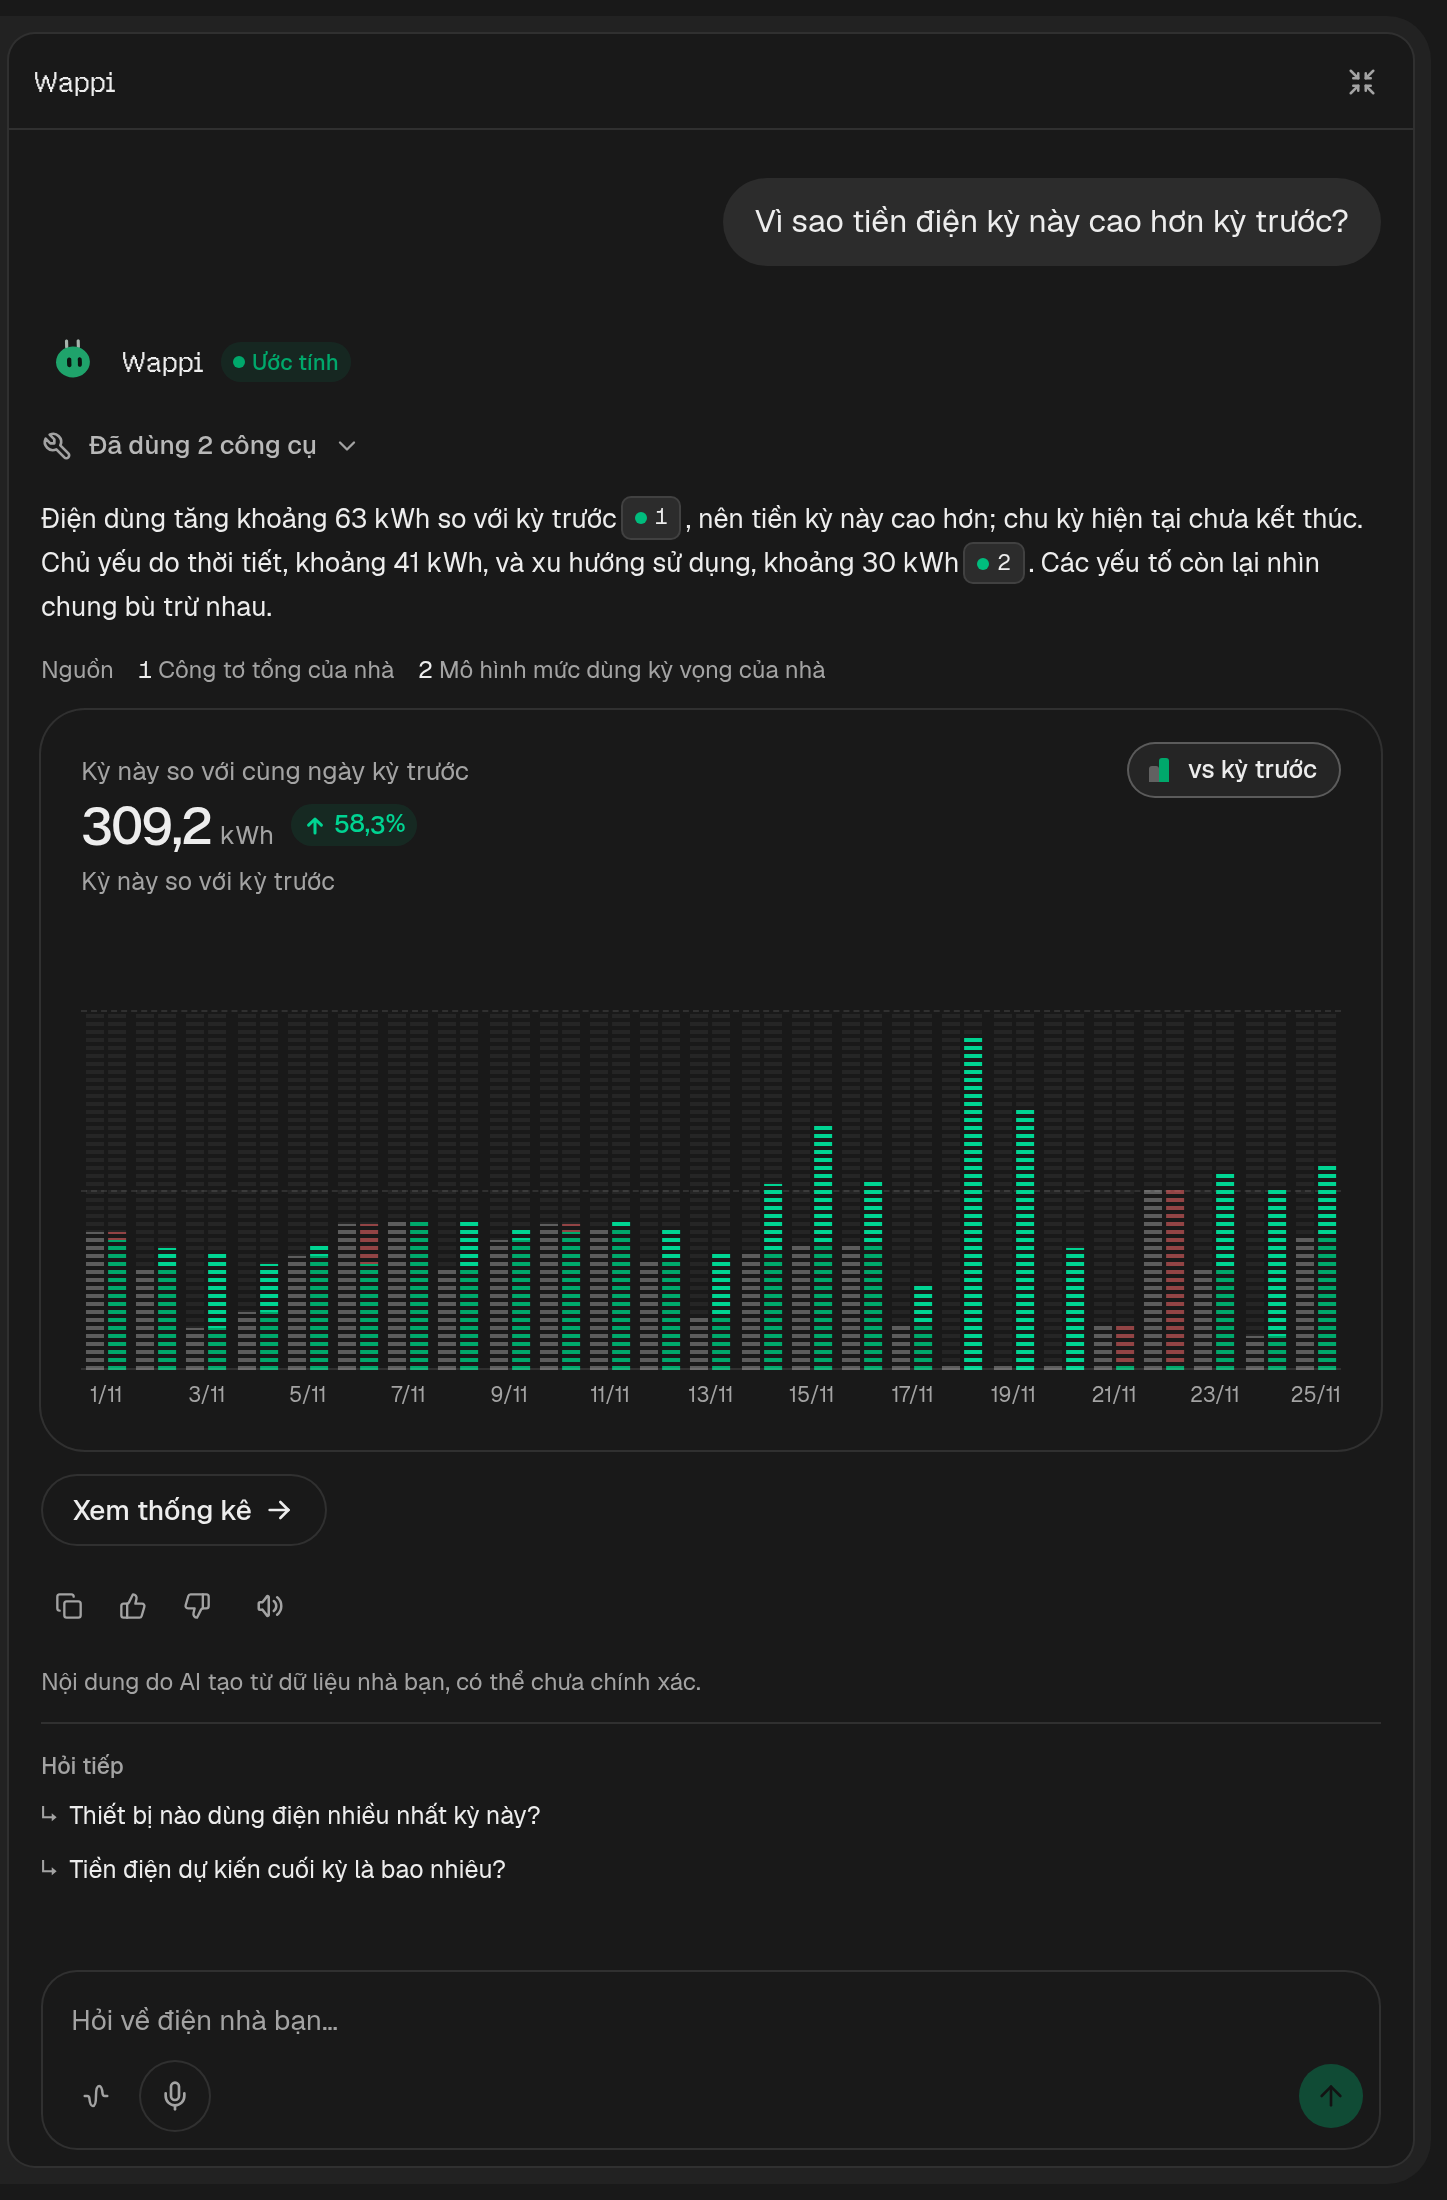
\includegraphics[height=6.6cm]{figures/q_d.png}\\
\small (c) Trò chuyện bằng giọng nói, đang nghe & \small (d) Câu trả lời kèm nguồn và biểu đồ
\end{tabular}
\caption{Trợ lý Wappi: 04 trạng thái. Ở (d), Wappi trả lời câu hỏi \emph{Vì sao tiền điện kỳ này cao hơn kỳ trước?} bằng số liệu từ 02 công cụ.}\label{fig:w4}
\end{figure}

\subsection{Minh bạch nguồn gốc giá trị hiển thị}\label{sec:minhbach}

Đề bài yêu cầu phân biệt rõ số đo được, số ước tính AI và dữ liệu minh họa. Độ tin cậy và cảnh báo chỉ hiện khi dữ liệu thiếu. Người dùng dễ nhầm số ước tính, số dự báo hoặc số của nhà demo với số đo thật. Nhóm tách các loại giá trị bằng nhãn trên giao diện (Bảng~\ref{tab:nhan}). Nhãn độ tin cậy chỉ gắn vào số do mô hình tạo ra. Khung cảnh báo chỉ hiện khi công tơ thiếu số đo.

\begin{table}[!ht]
\centering\caption{Các loại giá trị và nhãn tương ứng trên giao diện.}\label{tab:nhan}
\small\setlength{\tabcolsep}{4pt}\renewcommand{\arraystretch}{1.15}
\begin{tabularx}{\linewidth}{|>{\raggedright\arraybackslash}p{2.4cm}|>{\raggedright\arraybackslash}X|>{\raggedright\arraybackslash}X|>{\raggedright\arraybackslash}X|}
\hline
\textbf{Loại giá trị} & \textbf{Ví dụ} & \textbf{Nhãn trên giao diện} & \textbf{Khi nào hiện}\\
\hline
Đo được & Điện cả nhà, tiền điện đến hôm nay, hóa đơn các kỳ trước & Không gắn nhãn phụ. Trong Wappi gắn \emph{Đo trực tiếp} & Số lấy thẳng từ công tơ\\
\hline
Ước tính AI & Điện từng thiết bị, mục \emph{Khác} & \emph{Ước tính} kèm mức Cao, Vừa hoặc Thấp & Mọi số do NILM tạo ra\\
\hline
Dự báo & Hóa đơn cuối kỳ & \emph{Dự đoán} kèm mức tin cậy & Số chưa xảy ra\\
\hline
Dữ liệu minh họa & Nhà demo, kế hoạch mẫu & \emph{Nhà demo, chỉ xem} và nhãn \emph{Mẫu} & Mọi nhà demo\\
\hline
Dữ liệu thiếu & Hóa đơn kỳ này, từng kỳ trước & Khung \emph{Thiếu dữ liệu}, dòng \emph{Thiếu 18\% dữ liệu} & Công tơ có số đo dưới 95\% số phút của kỳ\\
\hline
\end{tabularx}
\end{table}

Mức tin cậy được tính riêng cho từng loại thiết bị từ kết quả kiểm tra của mô hình trên phần dữ liệu giữ lại. Giao diện chỉ hiện ba mức, không hiện điểm số. Mức Thấp kèm lời nhắc \emph{con số chỉ để tham khảo}. Wappi dùng 04 nhãn nguồn: \emph{Đo trực tiếp}, \emph{Theo văn bản}, \emph{Ước tính} và \emph{Suy luận bối cảnh} (Hình~\ref{fig:nhan2}).

\begin{figure}[H]\centering
\begin{tabular}{@{}c@{\hspace{4mm}}c@{\hspace{4mm}}c@{}}
\vtop{\hbox{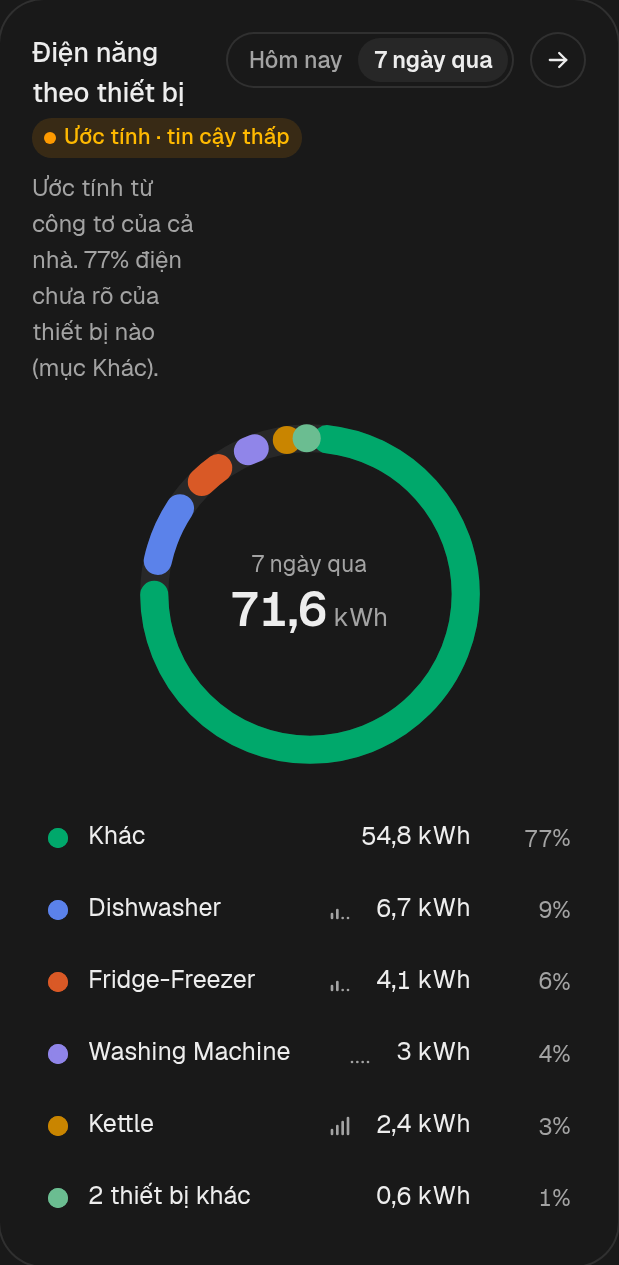
\includegraphics[width=4.4cm]{figures/n_uoc_tinh.png}}} & \vtop{\hbox{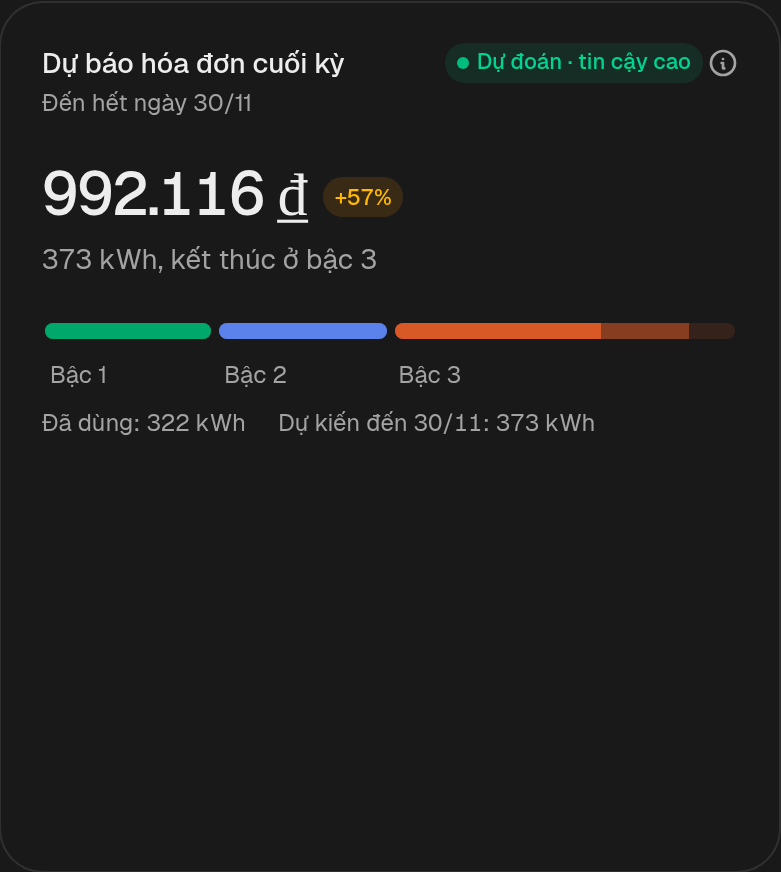
\includegraphics[width=5.4cm]{figures/n_du_doan.png}}} & \vtop{\hbox{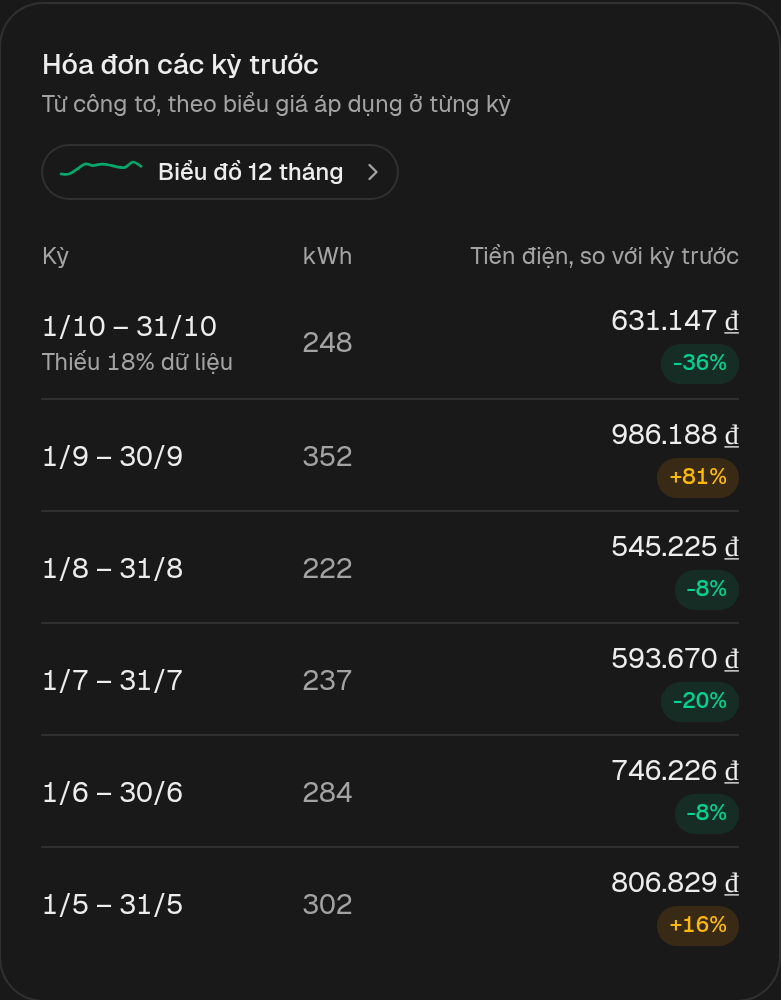
\includegraphics[width=5.4cm]{figures/n_thieu_ky.png}}}\\[3pt]
\parbox[t]{4.4cm}{\centering\small (a) Số ước tính AI: nhãn \emph{Ước tính, tin cậy thấp}} & \parbox[t]{5.4cm}{\centering\small (b) Số dự báo: nhãn \emph{Dự đoán, tin cậy cao}} & \parbox[t]{5.4cm}{\centering\small (c) Kỳ thiếu số đo: dòng \emph{Thiếu 18\% dữ liệu}}
\end{tabular}
\caption{Nhãn nguồn gốc và độ tin cậy trên các số do mô hình tạo ra và trên kỳ thiếu dữ liệu.}\label{fig:nhan1}
\end{figure}

\begin{figure}[H]\centering
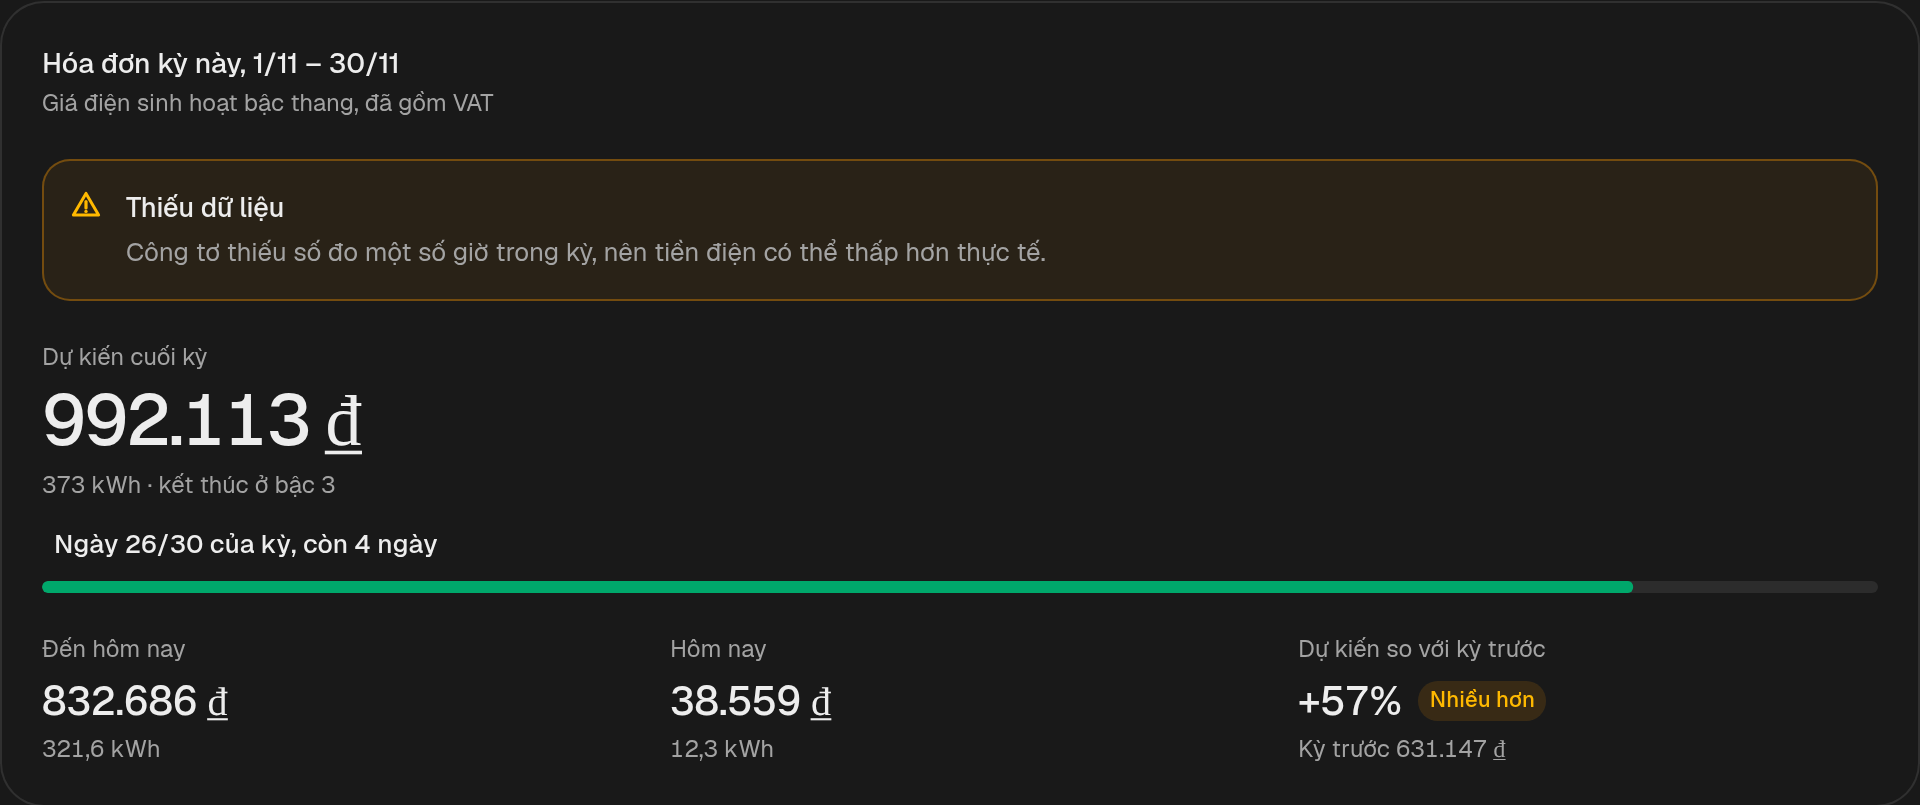
\includegraphics[width=.92\linewidth]{figures/n_thieu_hd.png}\\[2pt]{\small (d) Khung \emph{Thiếu dữ liệu} trên hóa đơn kỳ này}\\[8pt]
\begin{tabular}{@{}c@{\hspace{5mm}}c@{}}
\vtop{\hbox{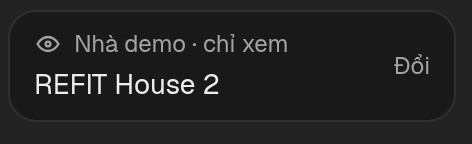
\includegraphics[width=4.6cm]{figures/n_demo.png}}} & \vtop{\hbox{
\includegraphics[width=10.4cm]{figures/tm_f.png}}}\\[3pt]
\small (e) Nhãn nhà demo & \small (f) Nhãn nguồn trong câu trả lời của Wappi
\end{tabular}
\caption{Khung cảnh báo thiếu dữ liệu, nhãn nhà demo và nhãn nguồn trong Wappi.}\label{fig:nhan2}
\end{figure}

Nhà REFIT House 2 có số đo bị thiếu thật. Kỳ 1/10 đến 31/10 thiếu 18\% dữ liệu và kỳ hiện tại thiếu một số giờ, nên các trạng thái thiếu dữ liệu xuất hiện tự nhiên. Nhóm chưa chèn nhiễu có chủ đích vào số đo. Việc này nằm trong bước tiếp theo.

\subsection{Chất lượng của Wappi}

Nhóm đánh giá Wappi ở 02 mốc (Bảng~\ref{tab:wappi}). Mốc 1 chạy trên 04 nhà demo và kiểm tra Wappi có đọc đúng con số từ công cụ không. Mốc 2 chạy trên REFIT House 2. Mốc 2 hỏi như người dùng thật, gồm 64 kịch bản chia thành 11 nhóm. Kết quả được chấm bằng kiểm tra tự động và 03 mô hình chấm độc lập (judge), không biết mô hình nào trả lời.

\begin{table}[!ht]
\centering\caption{Kết quả đo Wappi. Ở mốc 2, cột Sau là prompt phiên bản 3, mỗi bên một lượt.}\label{tab:wappi}
\small\setlength{\tabcolsep}{4pt}\renewcommand{\arraystretch}{1.15}
\begin{tabularx}{\linewidth}{|>{\raggedright\arraybackslash}X|>{\raggedleft\arraybackslash}p{2.2cm}|>{\raggedleft\arraybackslash}p{2.2cm}|}
\hline
\textbf{Chỉ số} & \textbf{Trước} & \textbf{Sau}\\
\hline
Mốc 1: câu đúng số liệu (84 câu, 4 nhà) & \multicolumn{2}{|r|}{84/84}\\
\hline
Mốc 1: thời gian đến chữ đầu tiên, trung vị & \multicolumn{2}{|r|}{khoảng 2 s}\\
\hline
Mốc 2: kiểm tra tự động đạt (64 câu) & 57/64 & 63/64\\
\hline
Mốc 2: câu về luật và biểu giá đạt (8 câu) & 2/8 & 8/8\\
\hline
Mốc 2: câu bị đánh giá khó nghe khi đọc to & 39 & 15\\
\hline
Mốc 2: câu mà đa số judge cho đạt & 55/64 & 45/64\\
\hline
\end{tabularx}
\end{table}

RAG đưa nhóm câu về luật từ 2/8 lên 8/8 và giảm một nửa số câu khó nghe khi đọc to. Đổi lại, câu trả lời ngắn hơn nên số câu được đa số judge cho đạt giảm từ 55 xuống 45 trên 64 câu. Nhóm đang chỉnh prompt để cân bằng giữa câu dễ nghe và câu đủ ý. Nhóm đã đo lại riêng nhóm câu nguyên nhân và nhóm câu mơ hồ. Nhóm xem đây là kết quả đánh giá nội bộ vì bộ kịch bản do nhóm viết. Mốc 1 chỉ đo việc đọc con số từ công cụ. Tập giữ lại đã được xem khi chỉnh prompt. Đánh giá độc lập là việc của giai đoạn thí điểm.

\subsection{Thay đổi so với bản cũ và bước tiếp theo}

\begin{table}[!ht]
\centering\caption{Thay đổi từ bản cũ đến web app Chặng 1.}\label{tab:changes}
\small\setlength{\tabcolsep}{4pt}\renewcommand{\arraystretch}{1.15}
\begin{tabularx}{\linewidth}{|>{\raggedright\arraybackslash}p{2.5cm}|>{\raggedright\arraybackslash}X|>{\raggedright\arraybackslash}X|}
\hline
 & \textbf{Bản cũ} & \textbf{Chặng 1}\\
\hline
Nền tảng & Bản mẫu trên điện thoại & Web app (dashboard và trang giới thiệu), chạy bằng Docker Compose\\
\hline
Dữ liệu & Số liệu minh họa & Bốn nhà demo dùng dữ liệu công khai, phát lại như công tơ thật\\
\hline
Hóa đơn & Biểu giá bậc thang minh họa & Tính theo QĐ 2892/QĐ-BCT, biểu giá lưu theo phiên bản ngày hiệu lực, dự báo cuối kỳ\\
\hline
Phân rã & Ý tưởng dùng NILMFormer & Worker \texttt{nilm} chạy nền, mô hình riêng từng nhà, đánh giá NILMFormer và 2Stage (mục~\ref{sec:nilm})\\
\hline
Trợ lý & Energy Copilot ở mức khái niệm & Wappi: 17 công cụ, RAG văn bản biểu giá, Text2SQL, giọng nói, nhãn nguồn gốc số liệu\\
\hline
Cảnh báo, kế hoạch & Mô tả trên bản mẫu & Cảnh báo tự động, kế hoạch tiết kiệm theo dõi đến cuối kỳ\\
\hline
Tài khoản & Không có & Đăng nhập Keycloak, đăng ký bằng email, khách xem thử không cần tài khoản\\
\hline
\end{tabularx}
\end{table}

Bước tiếp theo của nhóm gồm 06 việc:
\begin{enumerate}
\item Kiểm thử với số đo thiếu và nhiễu được chèn có chủ đích.
\item Thực nghiệm hiệu chỉnh theo hộ và ràng buộc tổng công suất như đã đề xuất trong hồ sơ.
\item Đưa 2Stage dùng chung vào ứng dụng.
\item Làm ứng dụng di động.
\item Thu số đo tại hộ Việt Nam.
\item Hợp tác với EVN.
\end{enumerate}
